\documentclass[a4paper,12pt]{article}

% -------------------------------------------------------------------------
% Paquetes
% -------------------------------------------------------------------------
\usepackage[utf8]{inputenc}
\usepackage[T1]{fontenc}
\usepackage[spanish,es-nodecimaldot,es-tabla]{babel}
\usepackage{lmodern}
\usepackage[margin=2.5cm]{geometry}
\usepackage{amsmath,amssymb}
\usepackage{graphicx}
\usepackage{subcaption}
\usepackage{booktabs}
\usepackage{xcolor}
\usepackage{palatino}
\usepackage[colorlinks=true,linkcolor=blue!60!black,citecolor=blue!60!black,urlcolor=blue!60!black]{hyperref}

%Add bibliography
\usepackage[sorting=none,style=phys]{biblatex}
\addbibresource{refs.bib}

% Figuras generadas por los scripts de analisis y de corridas
\graphicspath{{../analysis/output/}{../run/data/}}

% Notas para uno mismo durante la escritura (borrar antes de entregar)
\newcommand{\todo}[1]{\textcolor{red}{[\textbf{TODO:} #1]}}

% Notacion
\newcommand{\expval}[1]{\left\langle #1 \right\rangle}
\newcommand{\Tc}{T_c}

% -------------------------------------------------------------------------
\title{Simulaciones de Monte Carlo del modelo de Ising en $d = 2$\\[0.3em]
\large Elementos de la Teoría de los Fenómenos Críticos --- Guía N$^\circ$ 4}
\author{Nicolás Vazquez}
\date{\today}

\begin{document}
\maketitle

%\tableofcontents

% =========================================================================
\section{Introducción}
% =========================================================================
Dentro de la teoría del magnetismo y de los fenómenos críticos, el modelo de Ising es un sistema paradigmático \cite{tauberCriticalDynamicsField2014}.
Además de su importancia histórica, es un modelo simple que exhibe un comportamiento crítico que queda por fuera de las teorías ``clásicas'' de campo medio (como la teoría de Landau o Curie--Weiss) \cite{salinasIntroductionStatisticalPhysics2001}.

El modelo de Ising en dos dimensiones, con su transición de fase de segundo orden, es el modelo mínimo que caracteriza la transición paramagnética--ferromagnética de muchos materiales magnéticos \cite{blundellMagnetismCondensedMatter2023}. 
Sin embargo, en sentido estricto la transición de fase solo se da en el límite termodinámico: en un sistema finito las funciones termodinámicas son analíticas y no presentan singularidades \cite{goldenfeldLecturesPhaseTransitions2018}.
Si bien el modelo de Ising en dos dimensiones fue resuelto en este límite por Onsager \cite{Onsager1944}, la gran mayoría de los sistemas físicos no son tratables analíticamente, y por lo tanto se hace necesario recurrir a métodos numéricos para estudiar sus propiedades.

Las técnicas de Monte Carlo permiten hacer simulaciones numéricas de este sistema y de gran variedad de modelos afines, y son una herramienta fundamental para estudiar la física de los fenómenos críticos y del magnetismo en general \cite{landauGuideMonteCarlo2020}. 
Estos métodos, basados en la mecánica estadística de equilibrio y la teoría de los fenómenos críticos ---particularmente la teoría de escala y el análisis de tamaño finito \cite{cardy1988finite}---, permiten extrapolar los resultados obtenidos en sistemas finitos, como los de toda simulación, a la región crítica del límite termodinámico.

En este informe se presentan los resultados de simulaciones de Monte Carlo del modelo de Ising en la red cuadrada de dos dimensiones, con el objetivo de estudiar su comportamiento crítico: estimar la temperatura crítica y los exponentes críticos del modelo, y compararlos con los valores exactos conocidos.
% =========================================================================
\section{Modelo y método}
\label{sec:metodo}
% =========================================================================
En esta sección se describen brevemente la teoría del modelo de Ising, el algoritmo de Monte Carlo utilizado para simularlo, y los observables que se calcularon a partir de las simulaciones.
\subsection{Modelo}
El sistema que describe el modelo de Ising en dimensión $d=2$ consiste en un conjunto de espines $S_i = \pm 1$ ubicados en los sitios de una red cuadrada bidimensional de tamaño $L \times L$ (es decir $N = L^2$ sitios).
Estos espines interactúan con sus vecinos más cercanos (4 vecinos en la red cuadrada) y con un campo magnético externo $B$.
Sin entrar en detalles del fundamento detrás de cada término, la energía del sistema queda descrita por el Hamiltoniano \cite{salinasIntroductionStatisticalPhysics2001}
\begin{equation}
  H = -J \sum_{\langle i,j \rangle} S_i S_j - B \sum_i S_i ,
\end{equation}
donde $J$ es la constante de acoplamiento entre espines vecinos y $\langle i,j \rangle$ denota la suma sobre pares de sitios vecinos.
En el modelo de Ising ferromagnético, $J > 0$.

Lenz propuso este modelo en 1920 para estudiar el comportamiento de materiales ferromagnéticos, y su estudiante Ising lo resolvió en una dimensión en 1925, encontrando que no se da una transición de fase a temperatura finita. 
En cambio, a partir de la dimensión $d=2$ el modelo presenta orden ferromagnético a temperaturas suficientemente bajas y, por lo tanto, una transición de fase a una temperatura crítica $\Tc$ finita, algo demostrado por primera vez por Peierls en 1936 \cite{deoliveiraOriginsIsingModel2025}.

En un trabajo posterior, Onsager fue quien obtuvo la solución exacta del modelo de Ising en dos dimensiones en el límite termodinámico, que muestra que la transición es continua. 
Mencionamos debajo algunos resultados de la solución exacta que serán útiles para comparar con los resultados de las simulaciones.

\subsubsection{La solución exacta de Onsager}
Onsager resolvió el modelo a campo nulo mediante el método de la matriz de transferencia \cite{Onsager1944}.
La temperatura crítica queda determinada por la condición $\sinh(2J/k_B\Tc) = 1$, es decir
\begin{equation}
  \frac{k_B \Tc}{J} = \frac{2}{\ln\left(1 + \sqrt{2}\right)} \simeq 2.269185 .
\end{equation}
La magnetización espontánea, calculada posteriormente por Yang \cite{yangSpontaneousMagnetizationTwoDimensional1952}, es
\begin{equation}
  \expval{m} = \left[ 1 - \sinh^{-4}\left( \frac{2J}{k_B T} \right) \right]^{1/8}, \qquad T < \Tc ,
\end{equation}
y se anula de forma continua en $\Tc$.
Por su parte, el calor específico diverge logarítmicamente,
\begin{equation}
  \frac{C}{k_B} \simeq -\frac{8}{\pi} \left( \frac{J}{k_B \Tc} \right)^2 \ln\left| 1 - \frac{T}{\Tc} \right| ,
\end{equation}
por lo que $\alpha = 0$.
A partir de estos resultados y de la función de correlación exacta se obtienen los exponentes críticos
\begin{equation}
  \alpha = 0 \ (\text{log}), \quad \beta = \tfrac{1}{8}, \quad \gamma = \tfrac{7}{4}, \quad \nu = 1, \quad \eta = \tfrac{1}{4}, \quad \delta = 15 ,
\end{equation}
muy distintos de los de campo medio ($\beta = 1/2$, $\gamma = 1$, $\nu = 1/2$, $\eta = 0$, $\delta = 3$), y que definen la clase de universalidad de Ising en $d = 2$.
Estos son los valores con los que compararemos las estimaciones numéricas de la Sección~\ref{sec:resultados}.

\subsection{Algoritmo de Monte Carlo}
\label{sec:algoritmo}
Para muestrear la distribución de Boltzmann $P(\{S\}) \propto e^{-\beta H}$ se utilizó una dinámica de un solo espín con el algoritmo de baño térmico (\emph{heat bath}), también conocido como dinámica de Glauber \cite{landauGuideMonteCarlo2020}.
En cada paso elemental se elige un sitio $i$ al azar y se le asigna un nuevo valor, independiente del anterior, según la distribución de equilibrio condicionada a la configuración de sus vecinos:
\begin{equation}
  P(S_i = +1) = \frac{1}{1 + e^{-2\beta h_i}} , \qquad h_i = J \sum_{j \in \mathrm{v}(i)} S_j + B ,
  \label{eq:heatbath}
\end{equation}
donde $\mathrm{v}(i)$ son los 4 primeros vecinos de $i$.
Como la suma de los vecinos solo puede tomar los valores $0, \pm 2, \pm 4$, estas probabilidades se calculan una única vez para cada temperatura y se guardan en una tabla.
Se define un paso de Monte Carlo (MCS) como $N = L^2$ de estos intentos, de modo que en promedio cada espín es visitado una vez por MCS.
En todas las simulaciones se usaron condiciones de contorno periódicas y unidades $J = k_B = 1$.

El enunciado propone el algoritmo de Metropolis, en el que se propone invertir el espín y se acepta el cambio con probabilidad $\min(1, e^{-\beta \Delta E})$.
Ambos algoritmos satisfacen balance detallado respecto de la misma distribución,
\begin{equation}
  \frac{W(S_i \to -S_i)}{W(-S_i \to S_i)} = e^{-\beta \Delta E} ,
\end{equation}
por lo que conducen a los mismos promedios de equilibrio, y en consecuencia a las mismas estimaciones de $\Tc$ y de los exponentes estáticos.
Lo que cambia es la dinámica: como la probabilidad de cambio del baño térmico es siempre menor o igual que la de Metropolis, los tiempos de autocorrelación son algo mayores.
Sin embargo, es conocido que ambas dinámicas pertenecen a la misma clase de universalidad dinámica (modelo A), con exponente $z \simeq 2.17$ \cite{tauberCriticalDynamicsField2014}.

Por otra parte, la dinámica de Glauber tiene la ventaja de admitir una interpretación física directa: fue introducida como una ecuación maestra con tasas de transición que modelan el acoplamiento de los espines con un baño térmico \cite{glauberTimeDependentStatisticsIsing1963}, de modo que el tiempo medido en MCS puede interpretarse como un tiempo físico de relajación hacia el equilibrio.
En una dimensión este modelo es exactamente soluble, y la evolución de $\expval{S_i}$ obedece una ecuación de difusión discreta.

\subsection{Tiempos de autocorrelación y protocolo de muestreo}
\todo{Estimación de $\tau_\mathrm{int}$ con ventana autoconsistente; ralentización crítica; termalización $\max(500, \lceil 10\tau \rceil)$ y separación entre muestras $\max(2, \lceil 2.5\tau \rceil)$; muestras por temperatura.}

\begin{figure}[htbp]
  \centering
  \includegraphics[width=\textwidth]{decorrelation_L64_nT96.png}
  \caption{\todo{Autocorrelación de $|m|$ y $\tau_\mathrm{int}(T)$ (tests preliminares).}}
  \label{fig:decorrelacion}
\end{figure}

\subsection{Observables}
\todo{Definiciones de $\expval{|m|}$, $\chi'$, $C$, $\expval{m^2}$, $\expval{m^4}$, $U_L$; cálculo de errores.}
  \subsubsection{Susceptibilidad y calor específico como fluctuaciones}
  \label{sec:fluctuaciones}
  % =========================================================================
  \todo{Problema 1: derivación de}
  \begin{align}
    \chi &= \frac{\partial \expval{m}}{\partial B} = \beta N \left[ \expval{m^2} - \expval{m}^2 \right], \\
    C &= -T \frac{\partial^2 f}{\partial T^2} = \frac{\beta^2}{N} \left[ \expval{H^2} - \expval{H}^2 \right].
  \end{align}
  % =========================================================================
% =========================================================================
\section{Resultados}
\label{sec:resultados}
% =========================================================================

\subsection{Curvas termodinámicas a campo nulo}
\label{sec:curvas}
\todo{Ítem (a).}

\begin{figure}[htbp]
  \centering
  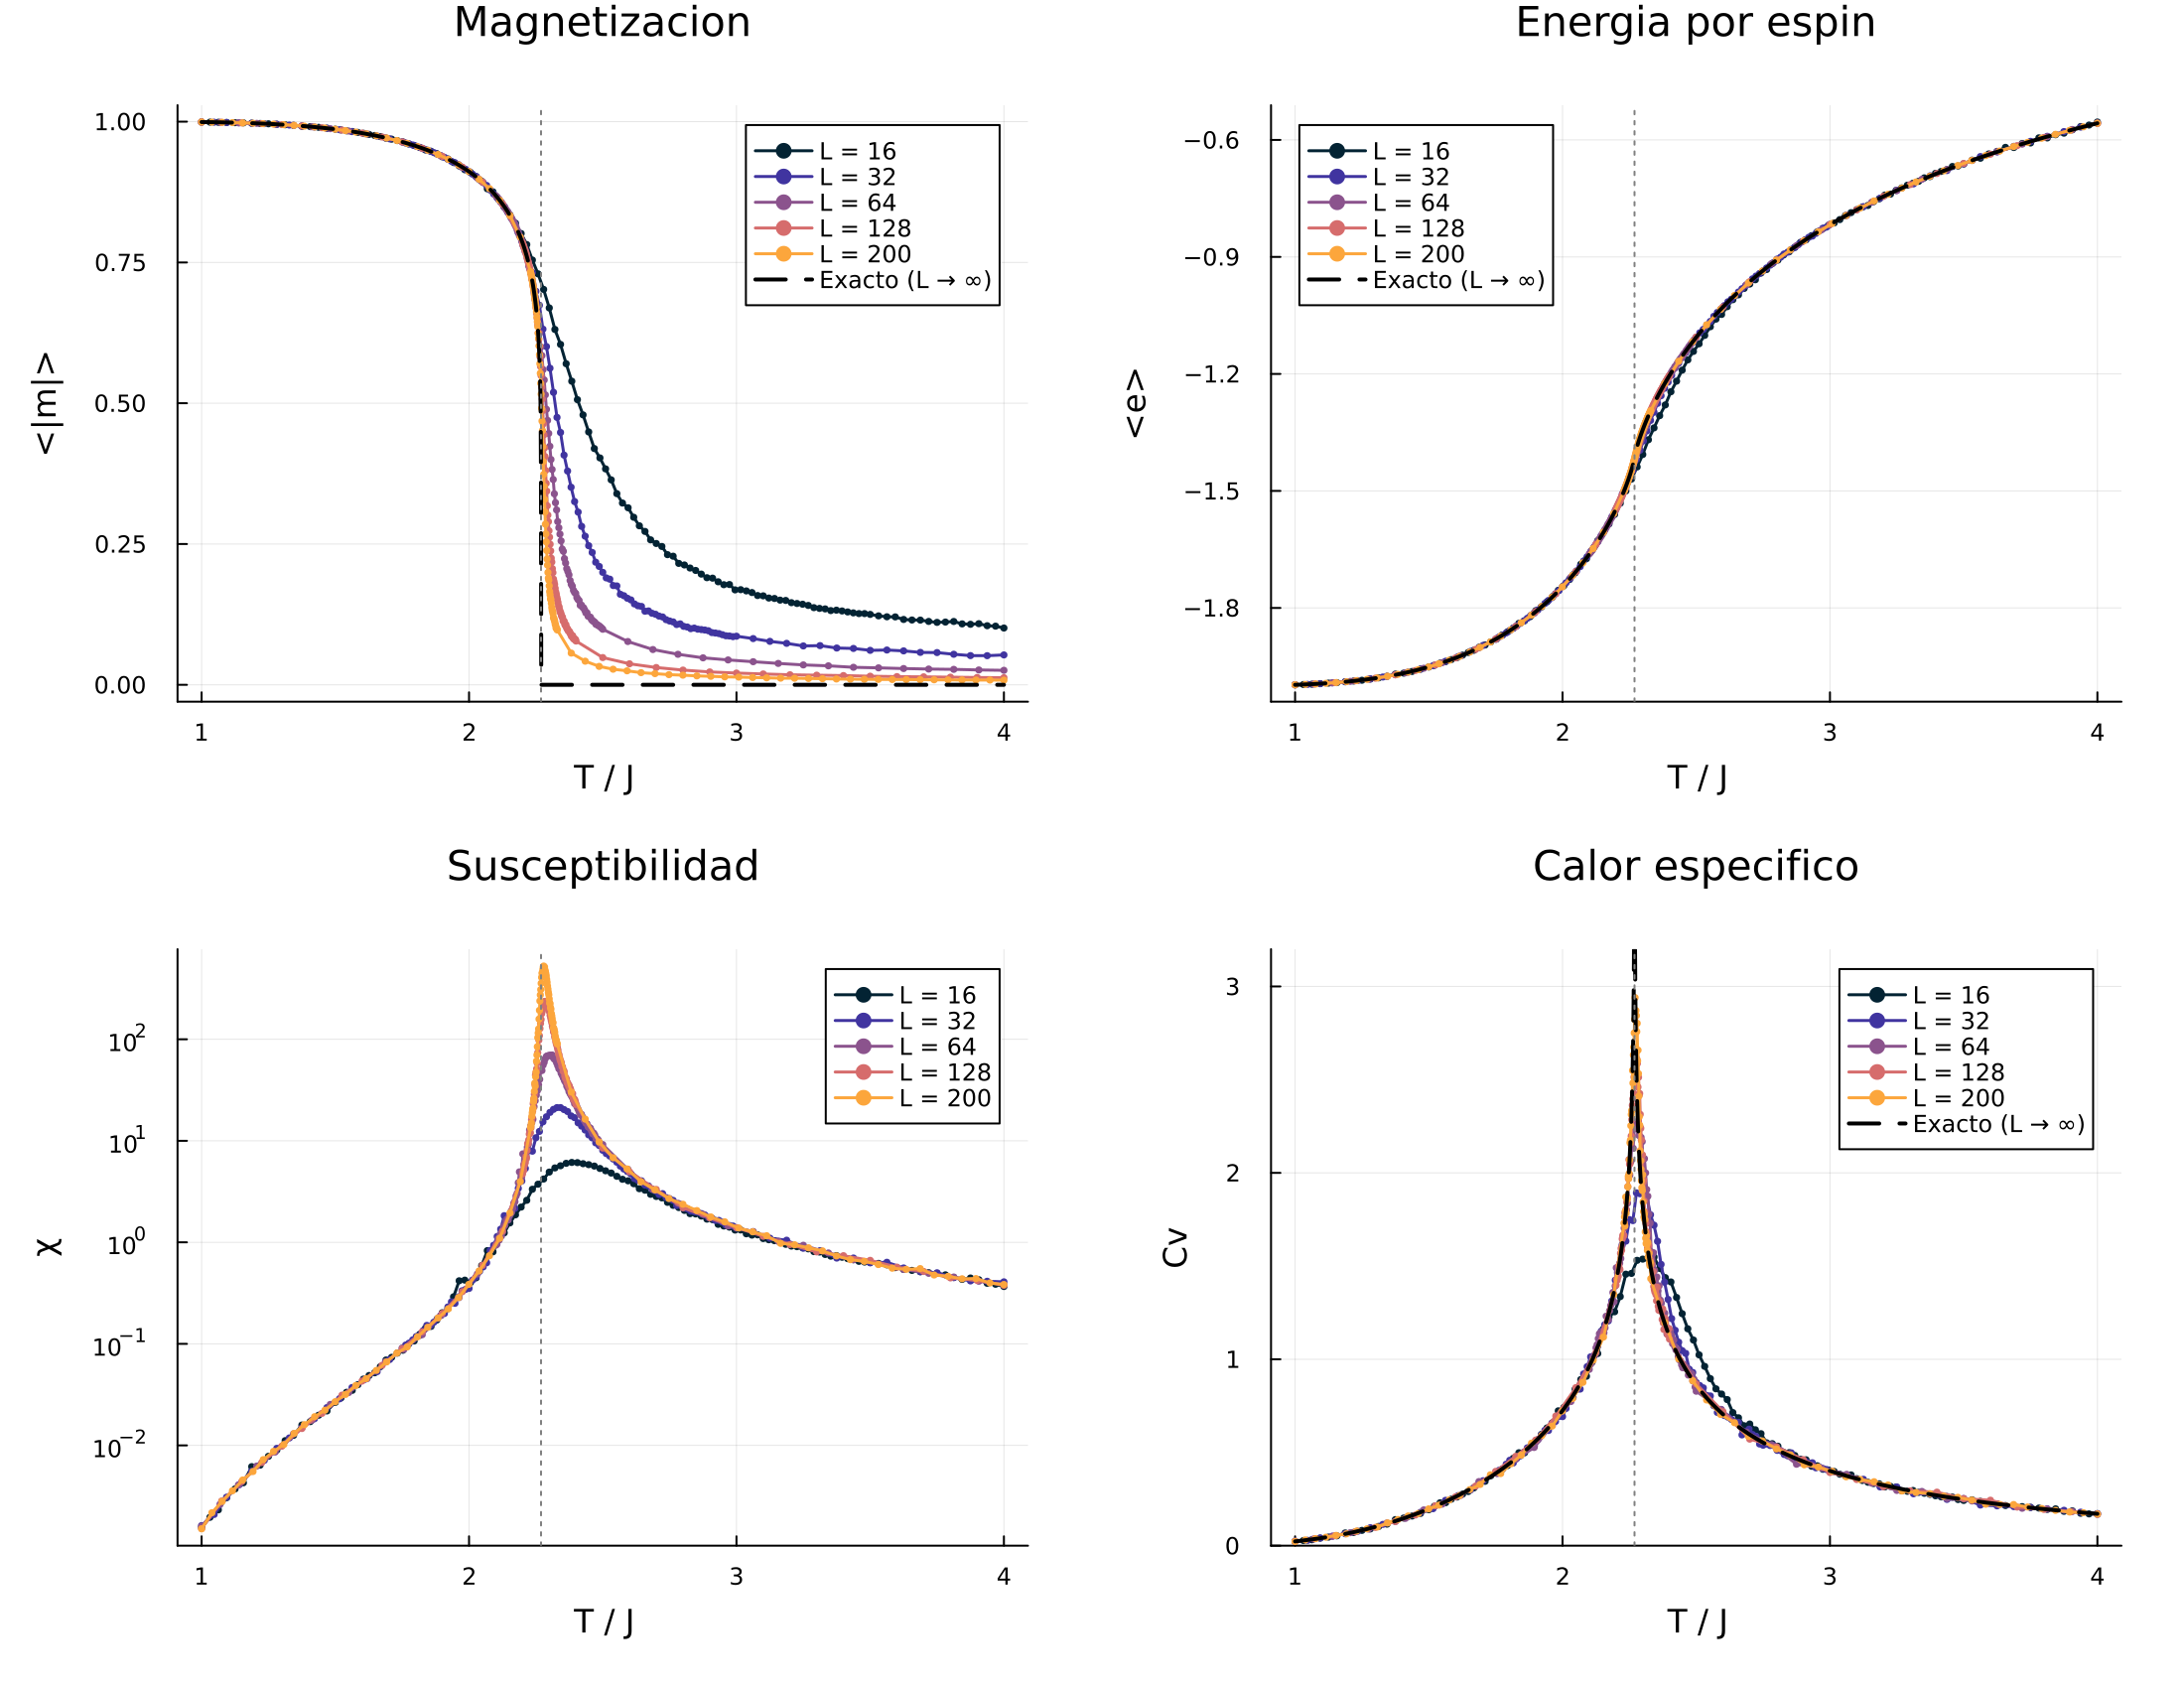
\includegraphics[width=\textwidth]{observables_vs_exact.png}
  \caption{\todo{$\expval{|m|}$, $\expval{e}$, $\chi$ y $C$ para $L = 16, 32, 64, 128, 200$, con la solución exacta de red infinita.}}
  \label{fig:observables}
\end{figure}

\begin{figure}[htbp]
  \centering
  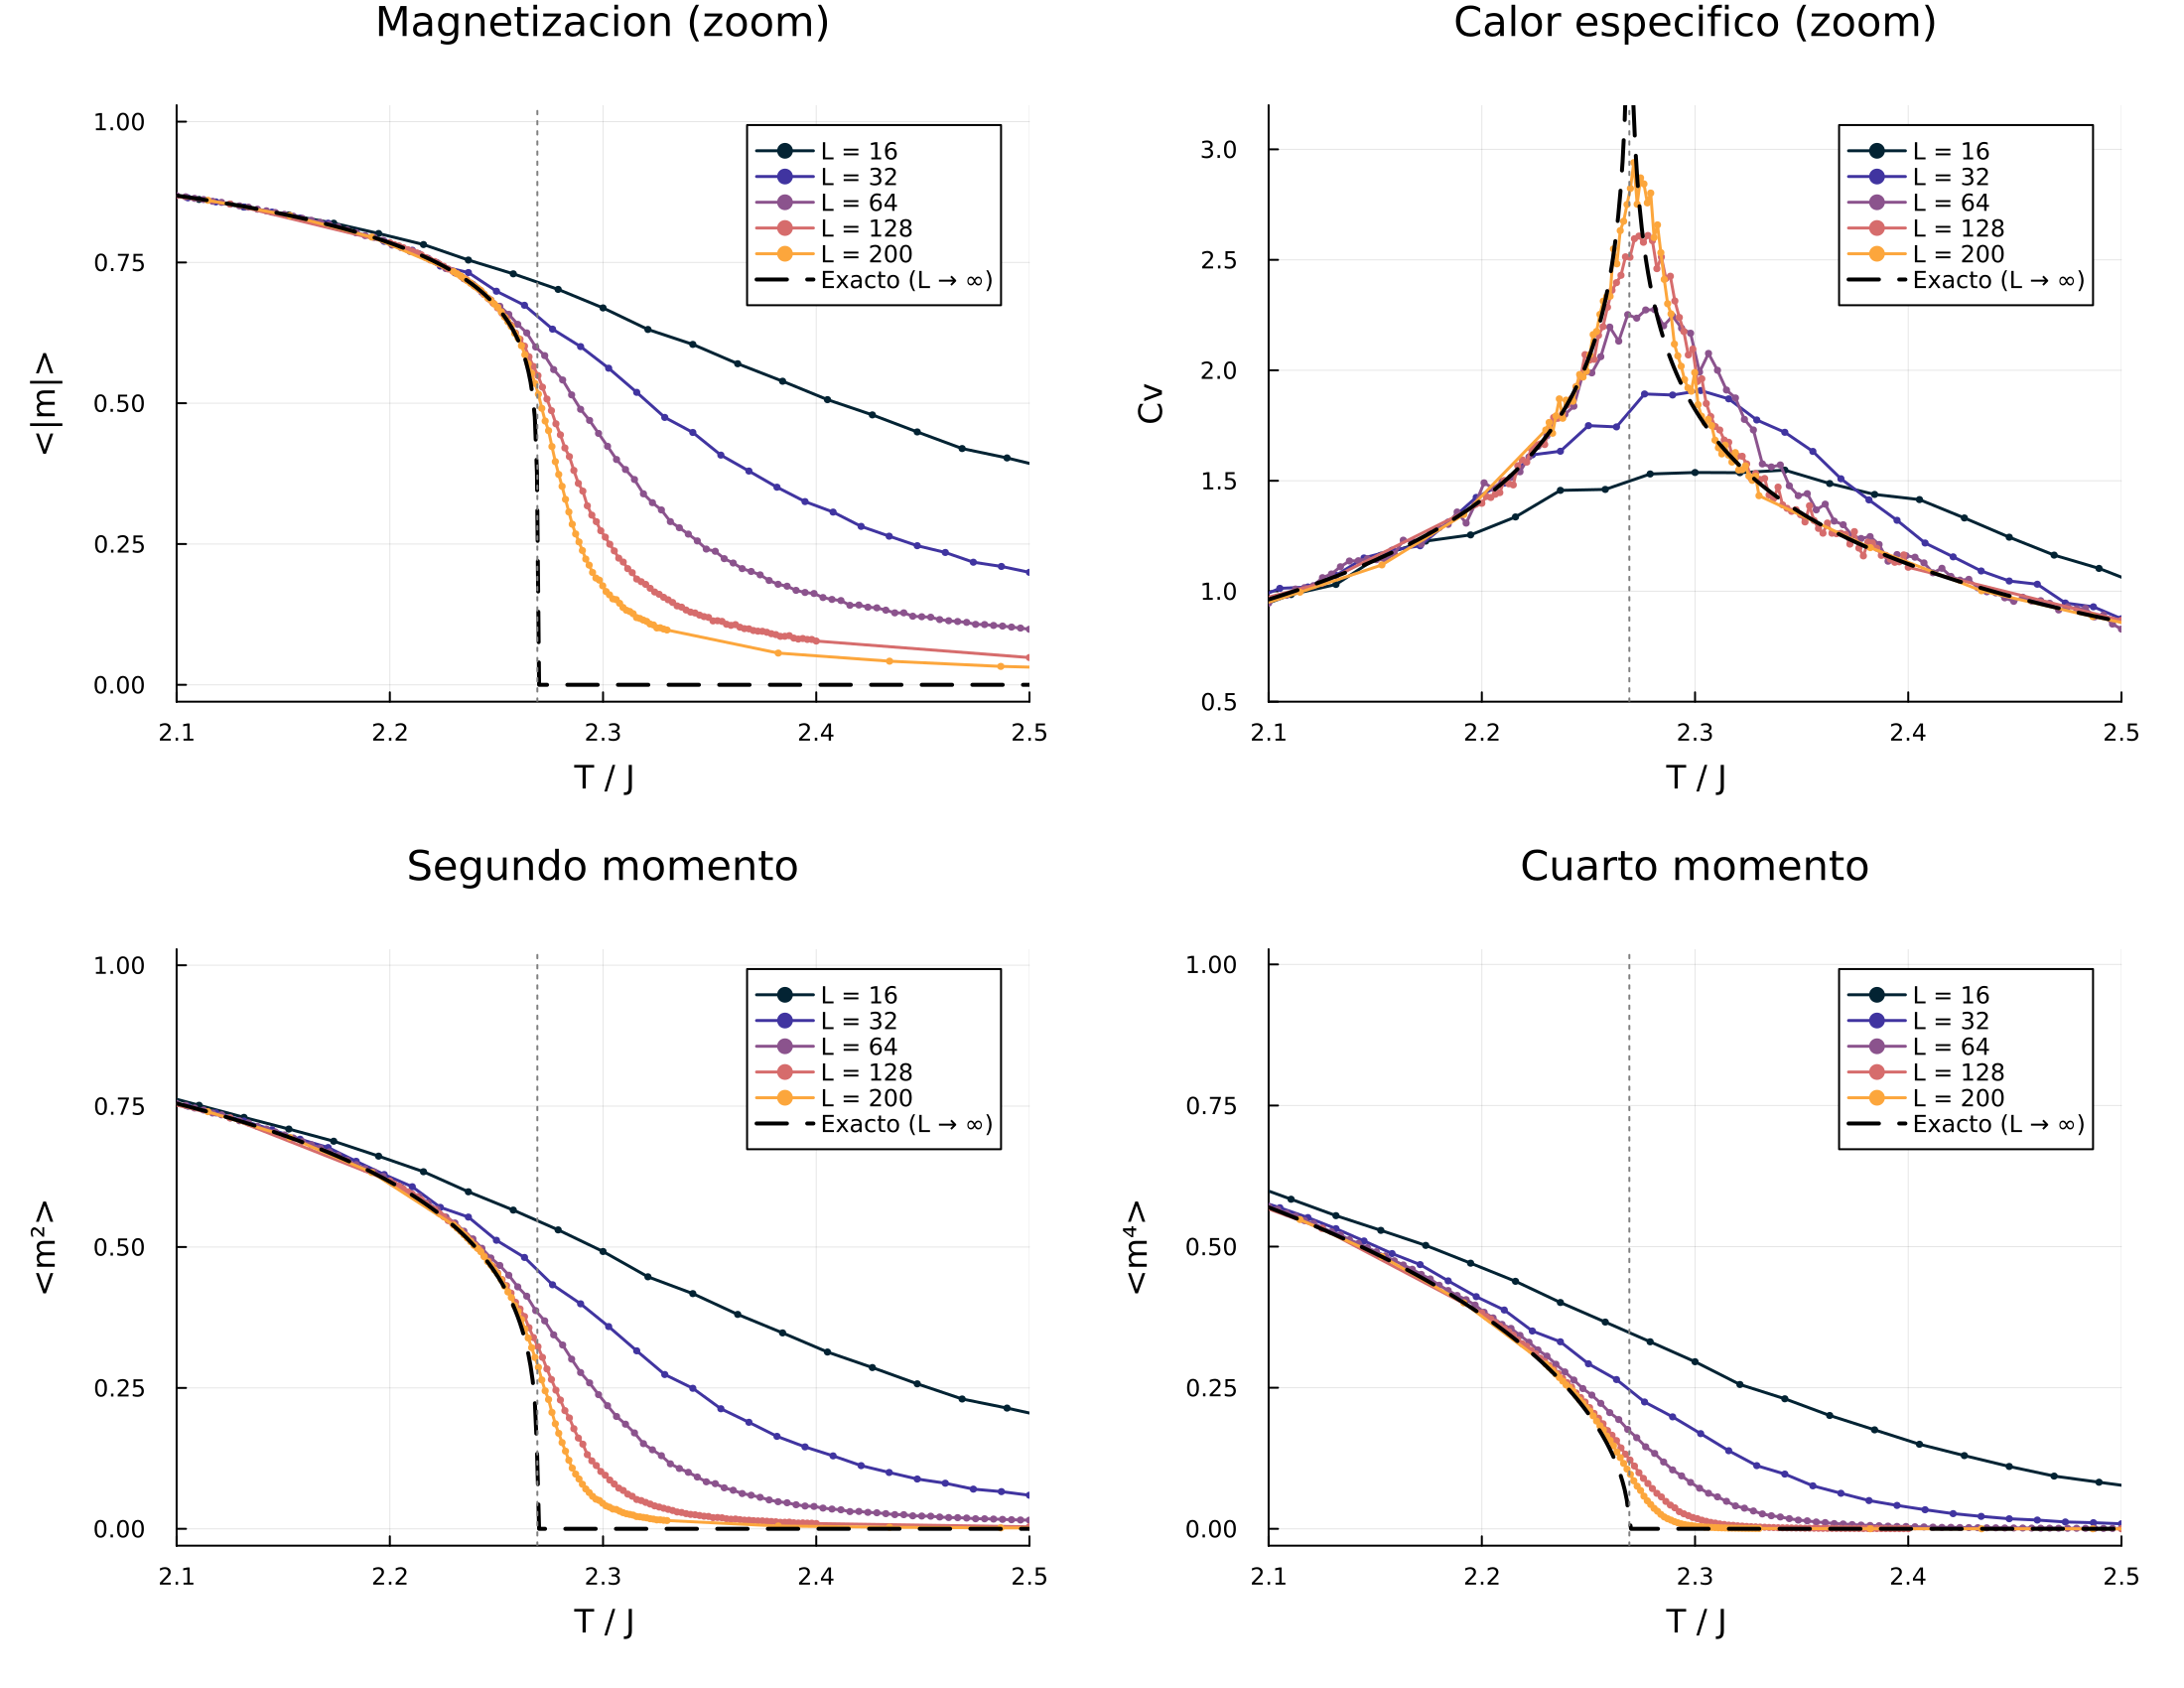
\includegraphics[width=\textwidth]{observables_near_Tc.png}
  \caption{\todo{Zoom en la región crítica y momentos $\expval{m^2}_L$, $\expval{m^4}_L$.}}
  \label{fig:observables_zoom}
\end{figure}

\subsection{Punto de inflexión de la magnetización}
\label{sec:inflexion}
\todo{Ítem (b): extrapolación $1/L \to 0$ y saturación $\propto 1/\sqrt{N}$.}

\begin{figure}[htbp]
  \centering
  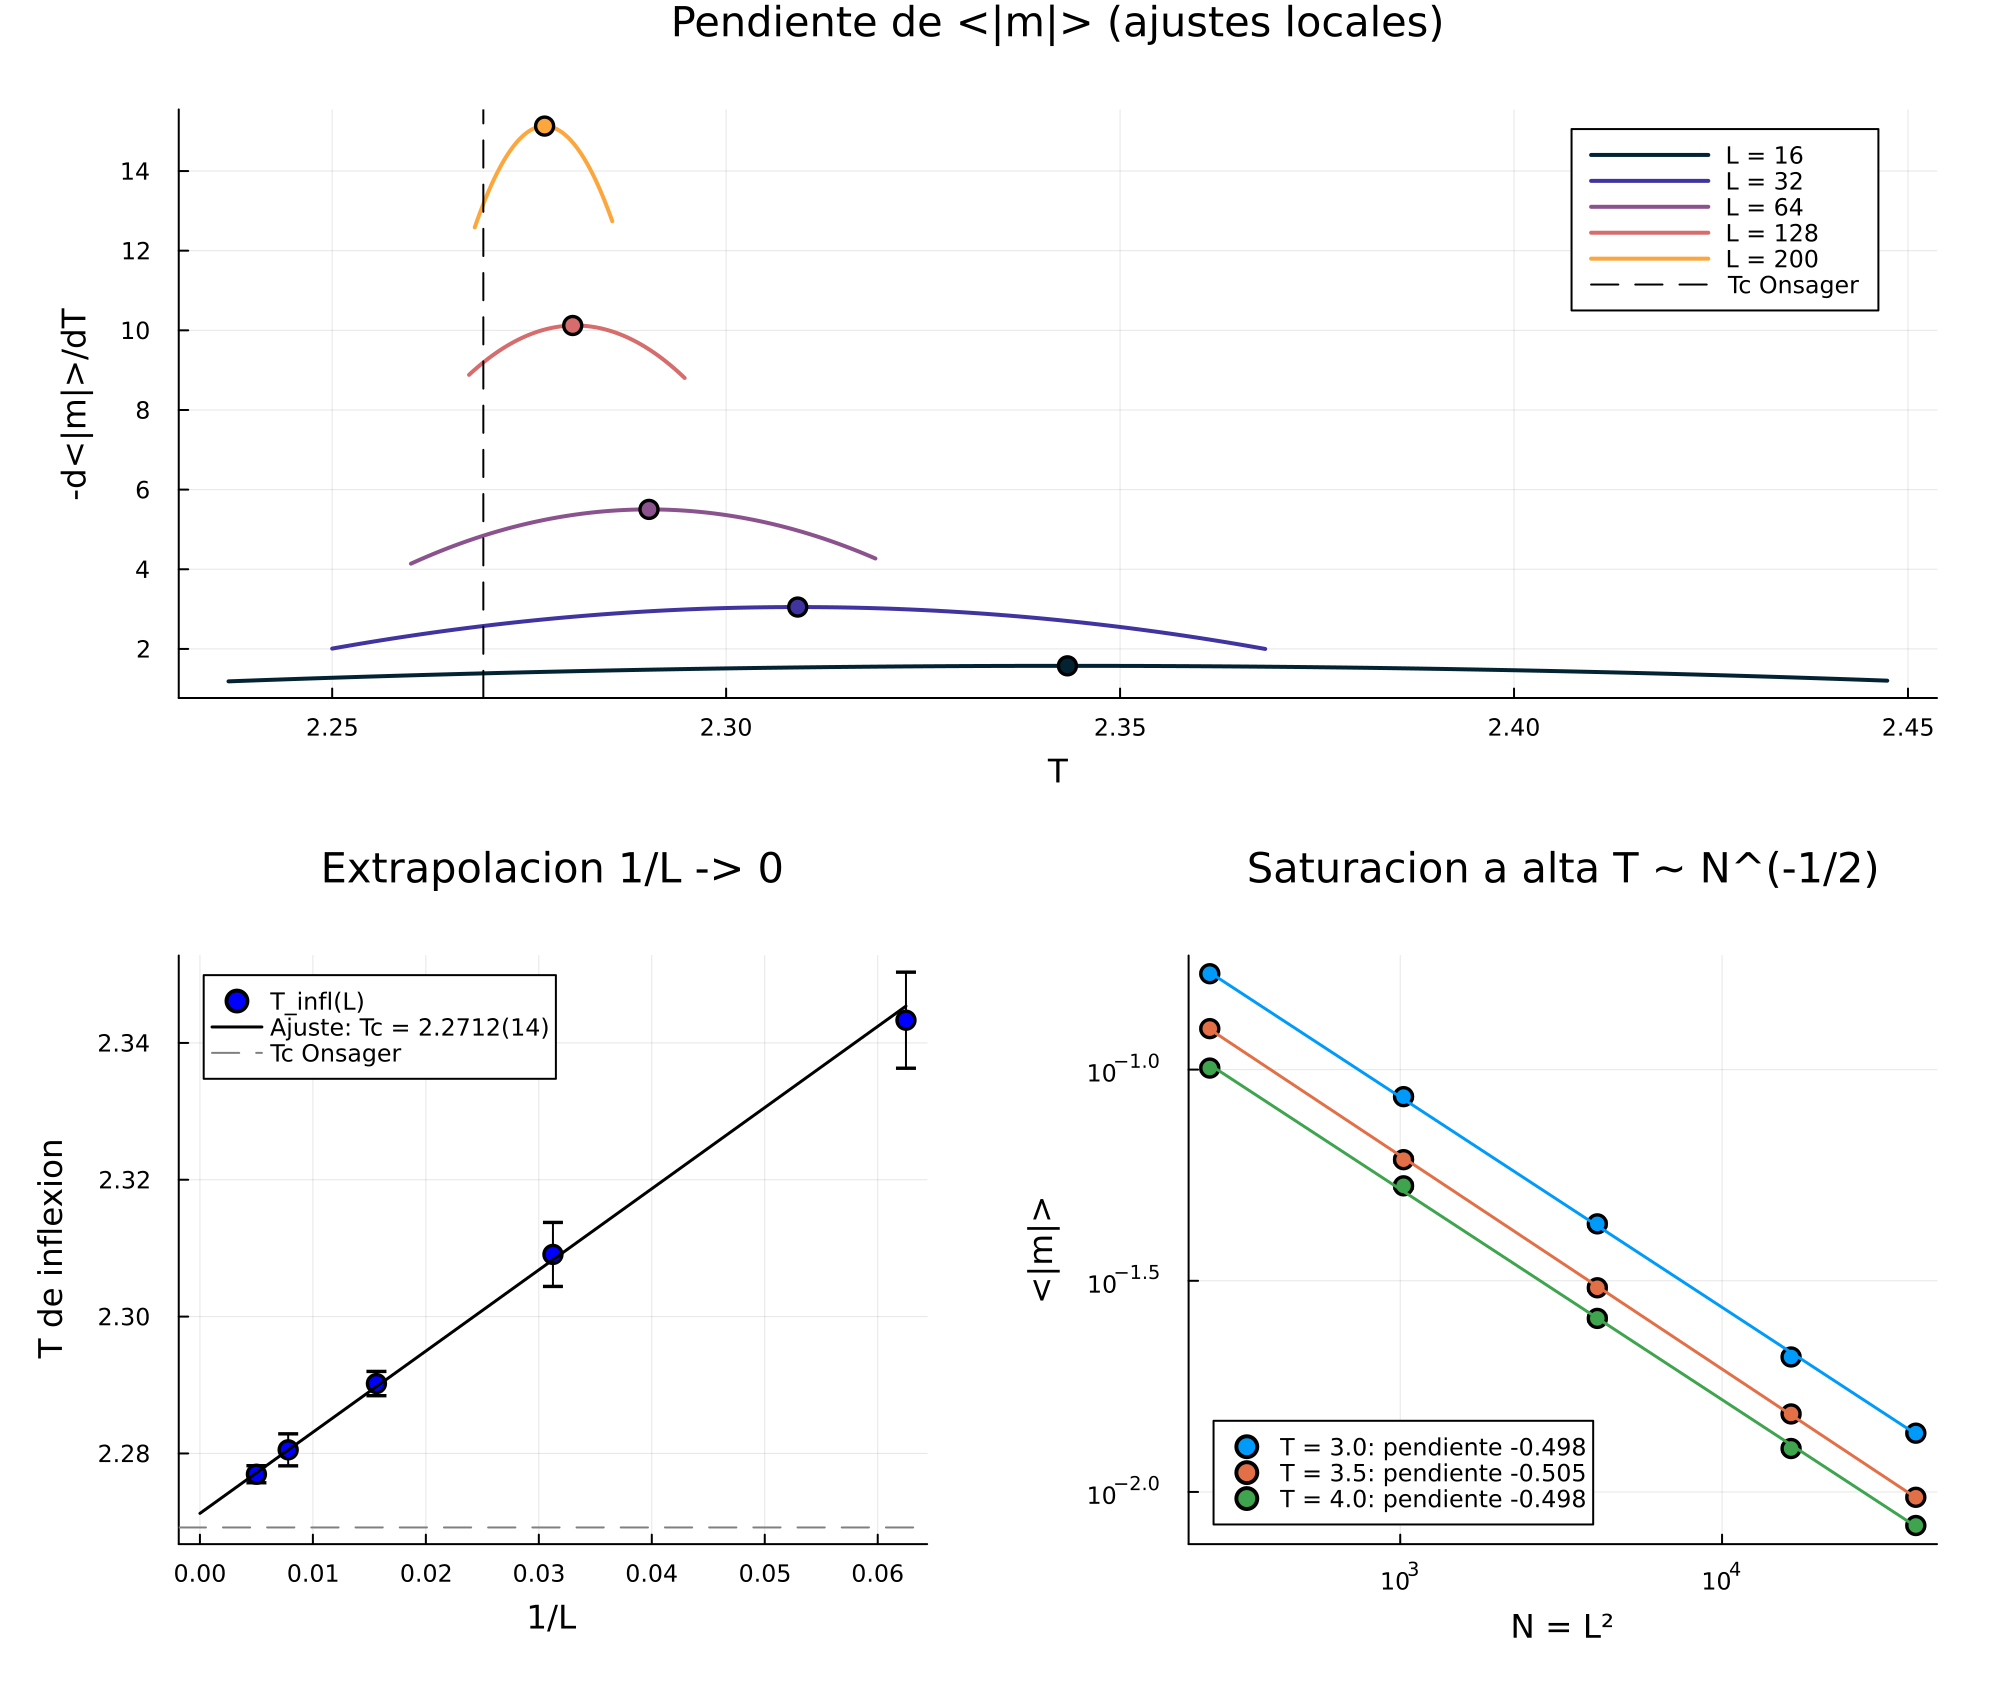
\includegraphics[width=\textwidth]{magnetization_inflection.png}
  \caption{\todo{Punto de inflexión de $\expval{|m|}$, extrapolación y saturación a alta $T$.}}
  \label{fig:inflexion}
\end{figure}

\subsection{Cumulante de Binder}
\label{sec:binder}
\todo{Ítem (c).}

\begin{figure}[htbp]
  \centering
  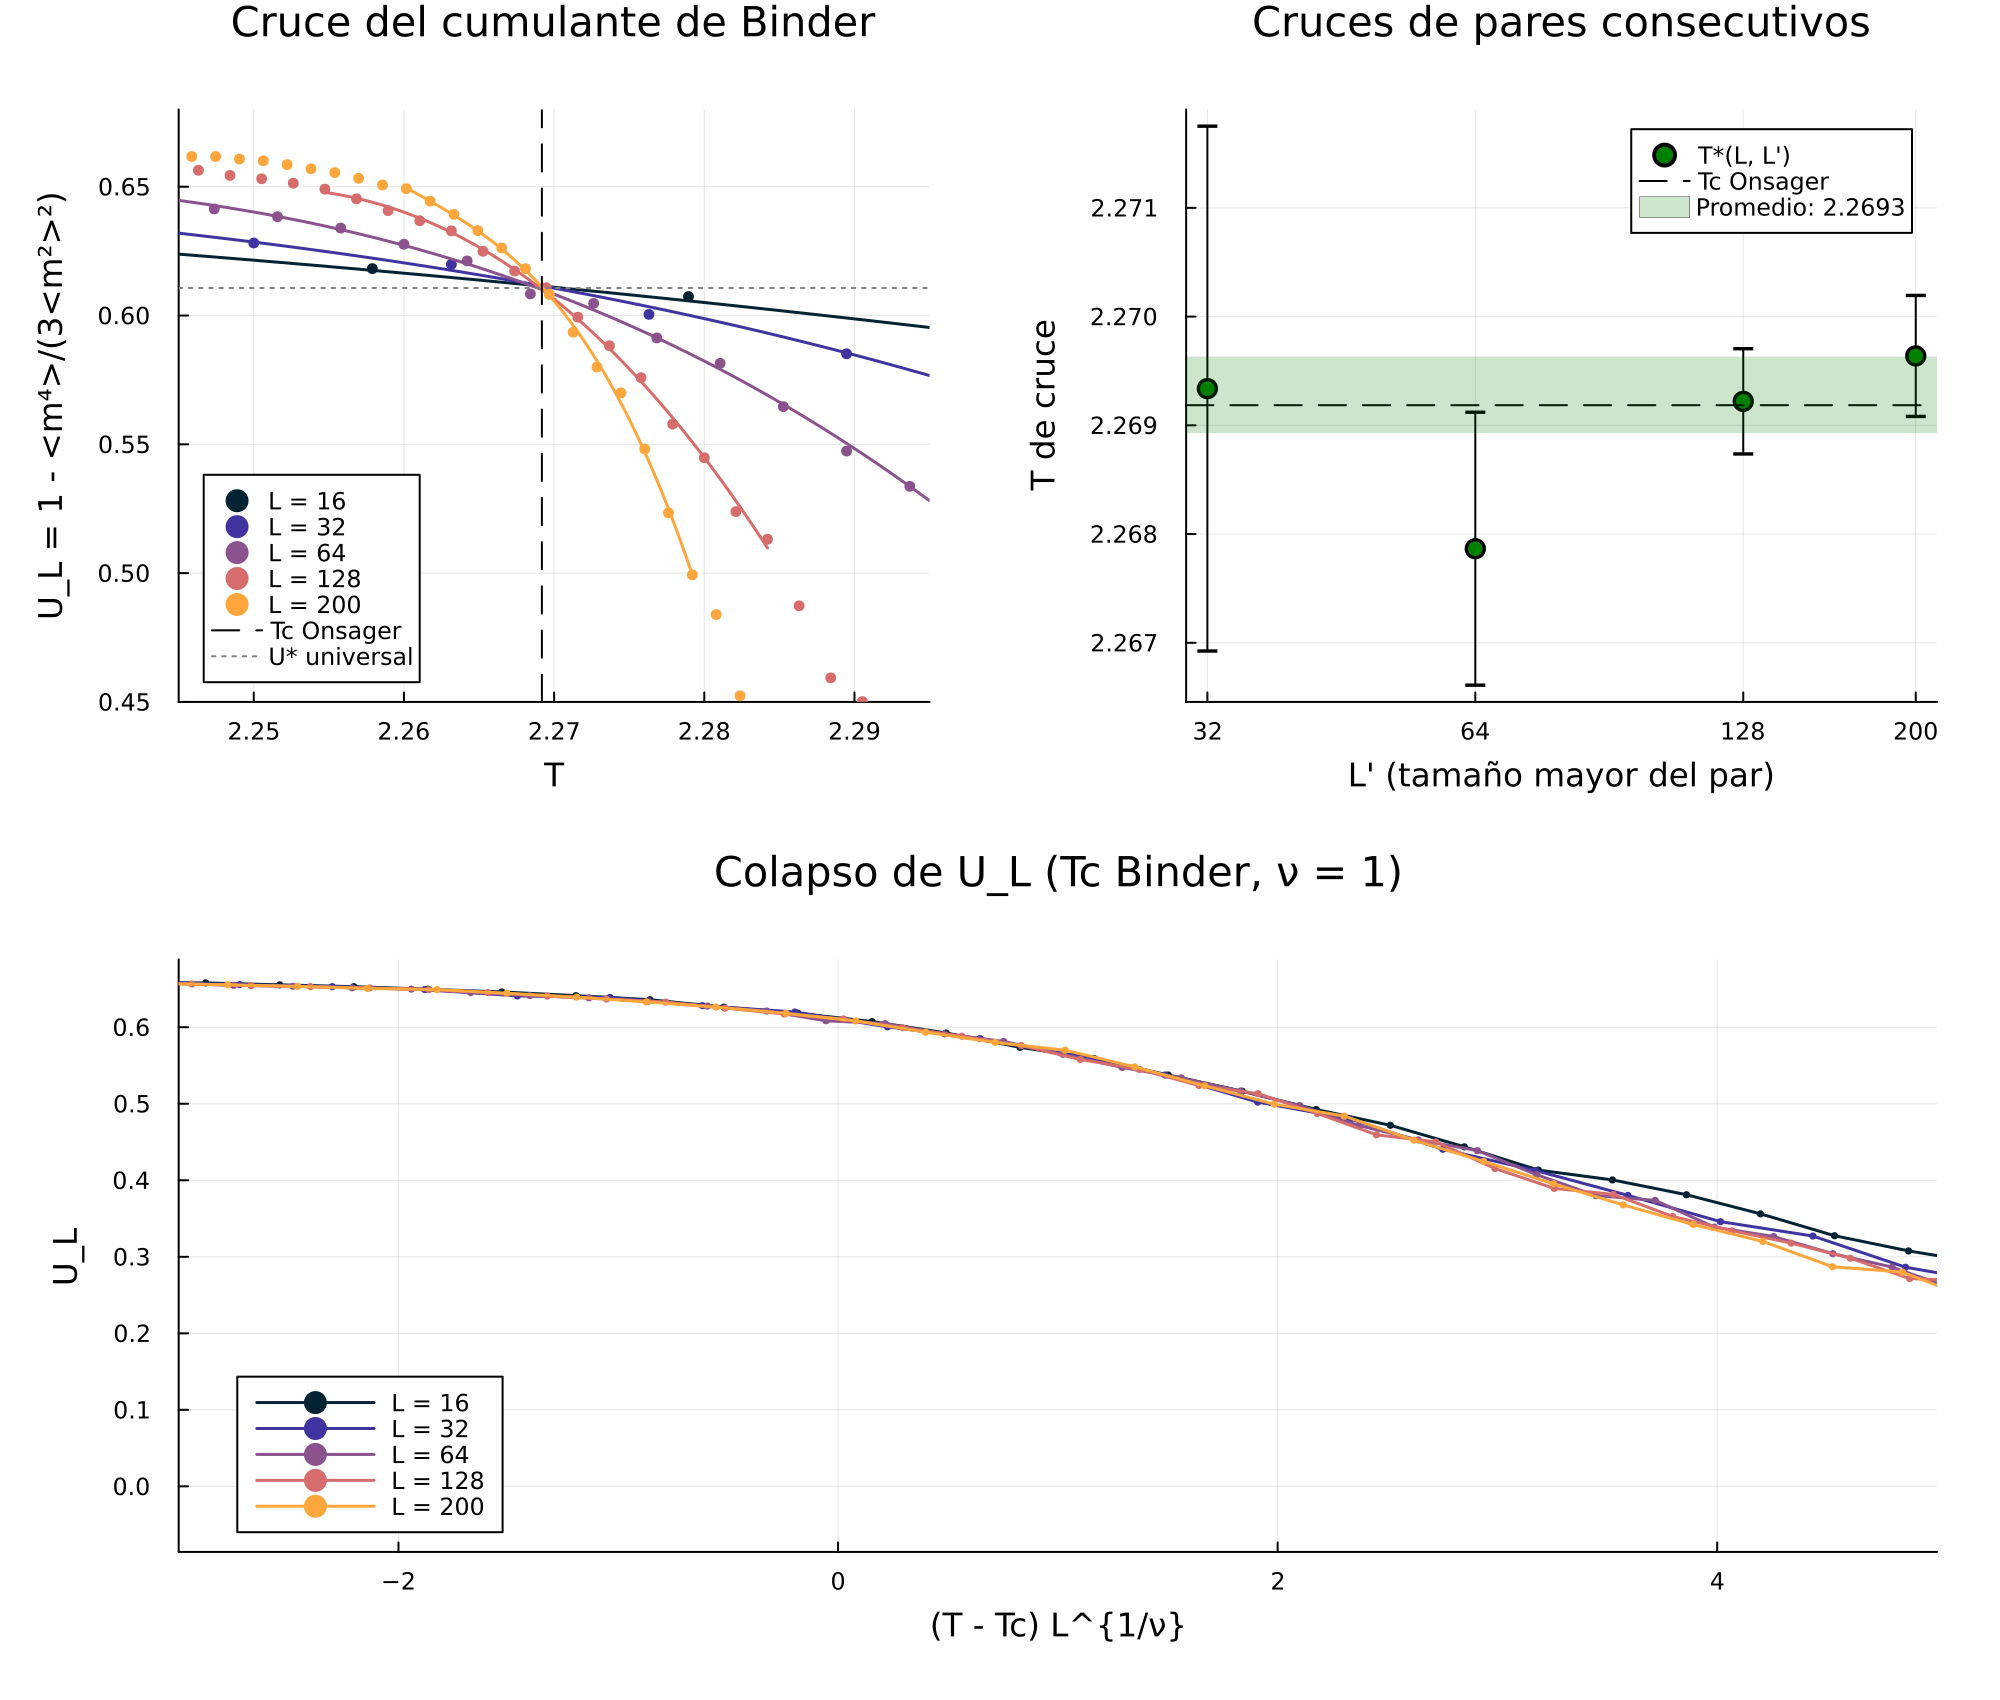
\includegraphics[width=\textwidth]{binder_crossing.png}
  \caption{\todo{Cruce del cumulante de Binder.}}
  \label{fig:binder}
\end{figure}

\subsection{Máximo de la susceptibilidad}
\label{sec:chi}
\todo{Ítem (d): $T^*(L) = \Tc + A L^{-1/\nu}$ y $\chi_\mathrm{max} \sim L^{\gamma/\nu}$.}

\begin{figure}[htbp]
  \centering
  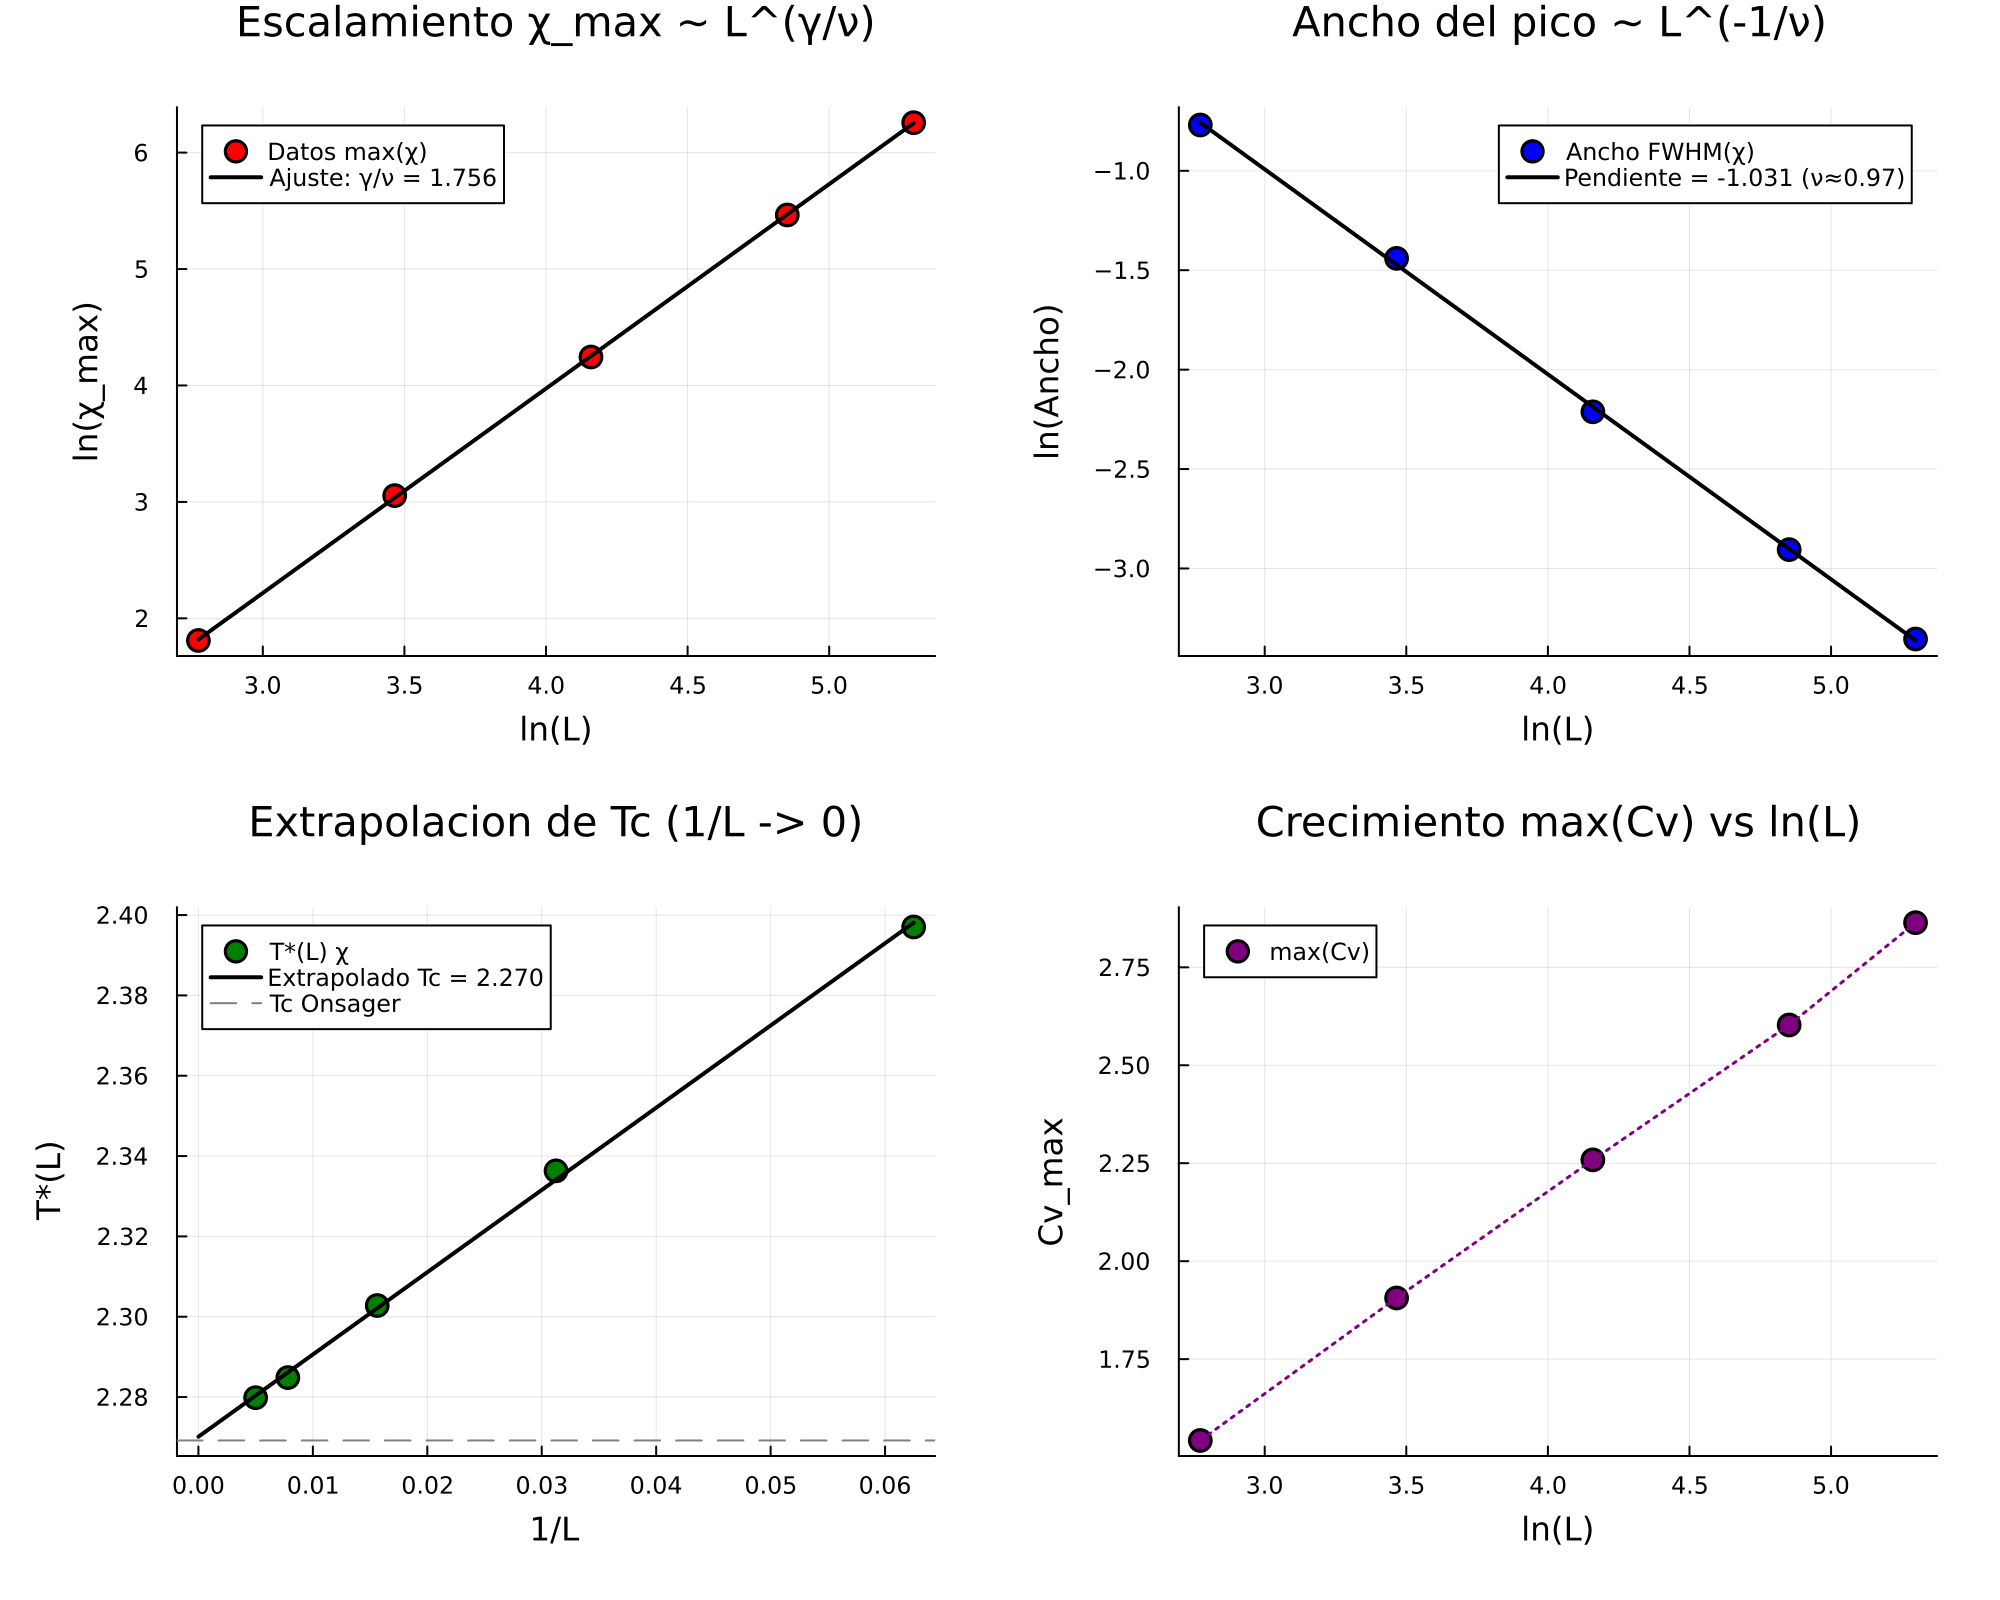
\includegraphics[width=\textwidth]{fss_scaling_fits.png}
  \caption{\todo{Escalamiento de tamaño finito del pico de $\chi$.}}
  \label{fig:chi}
\end{figure}

\subsection{Exponentes críticos}
\label{sec:exponentes}
\todo{Ítem (e).}

\begin{figure}[htbp]
  \centering
  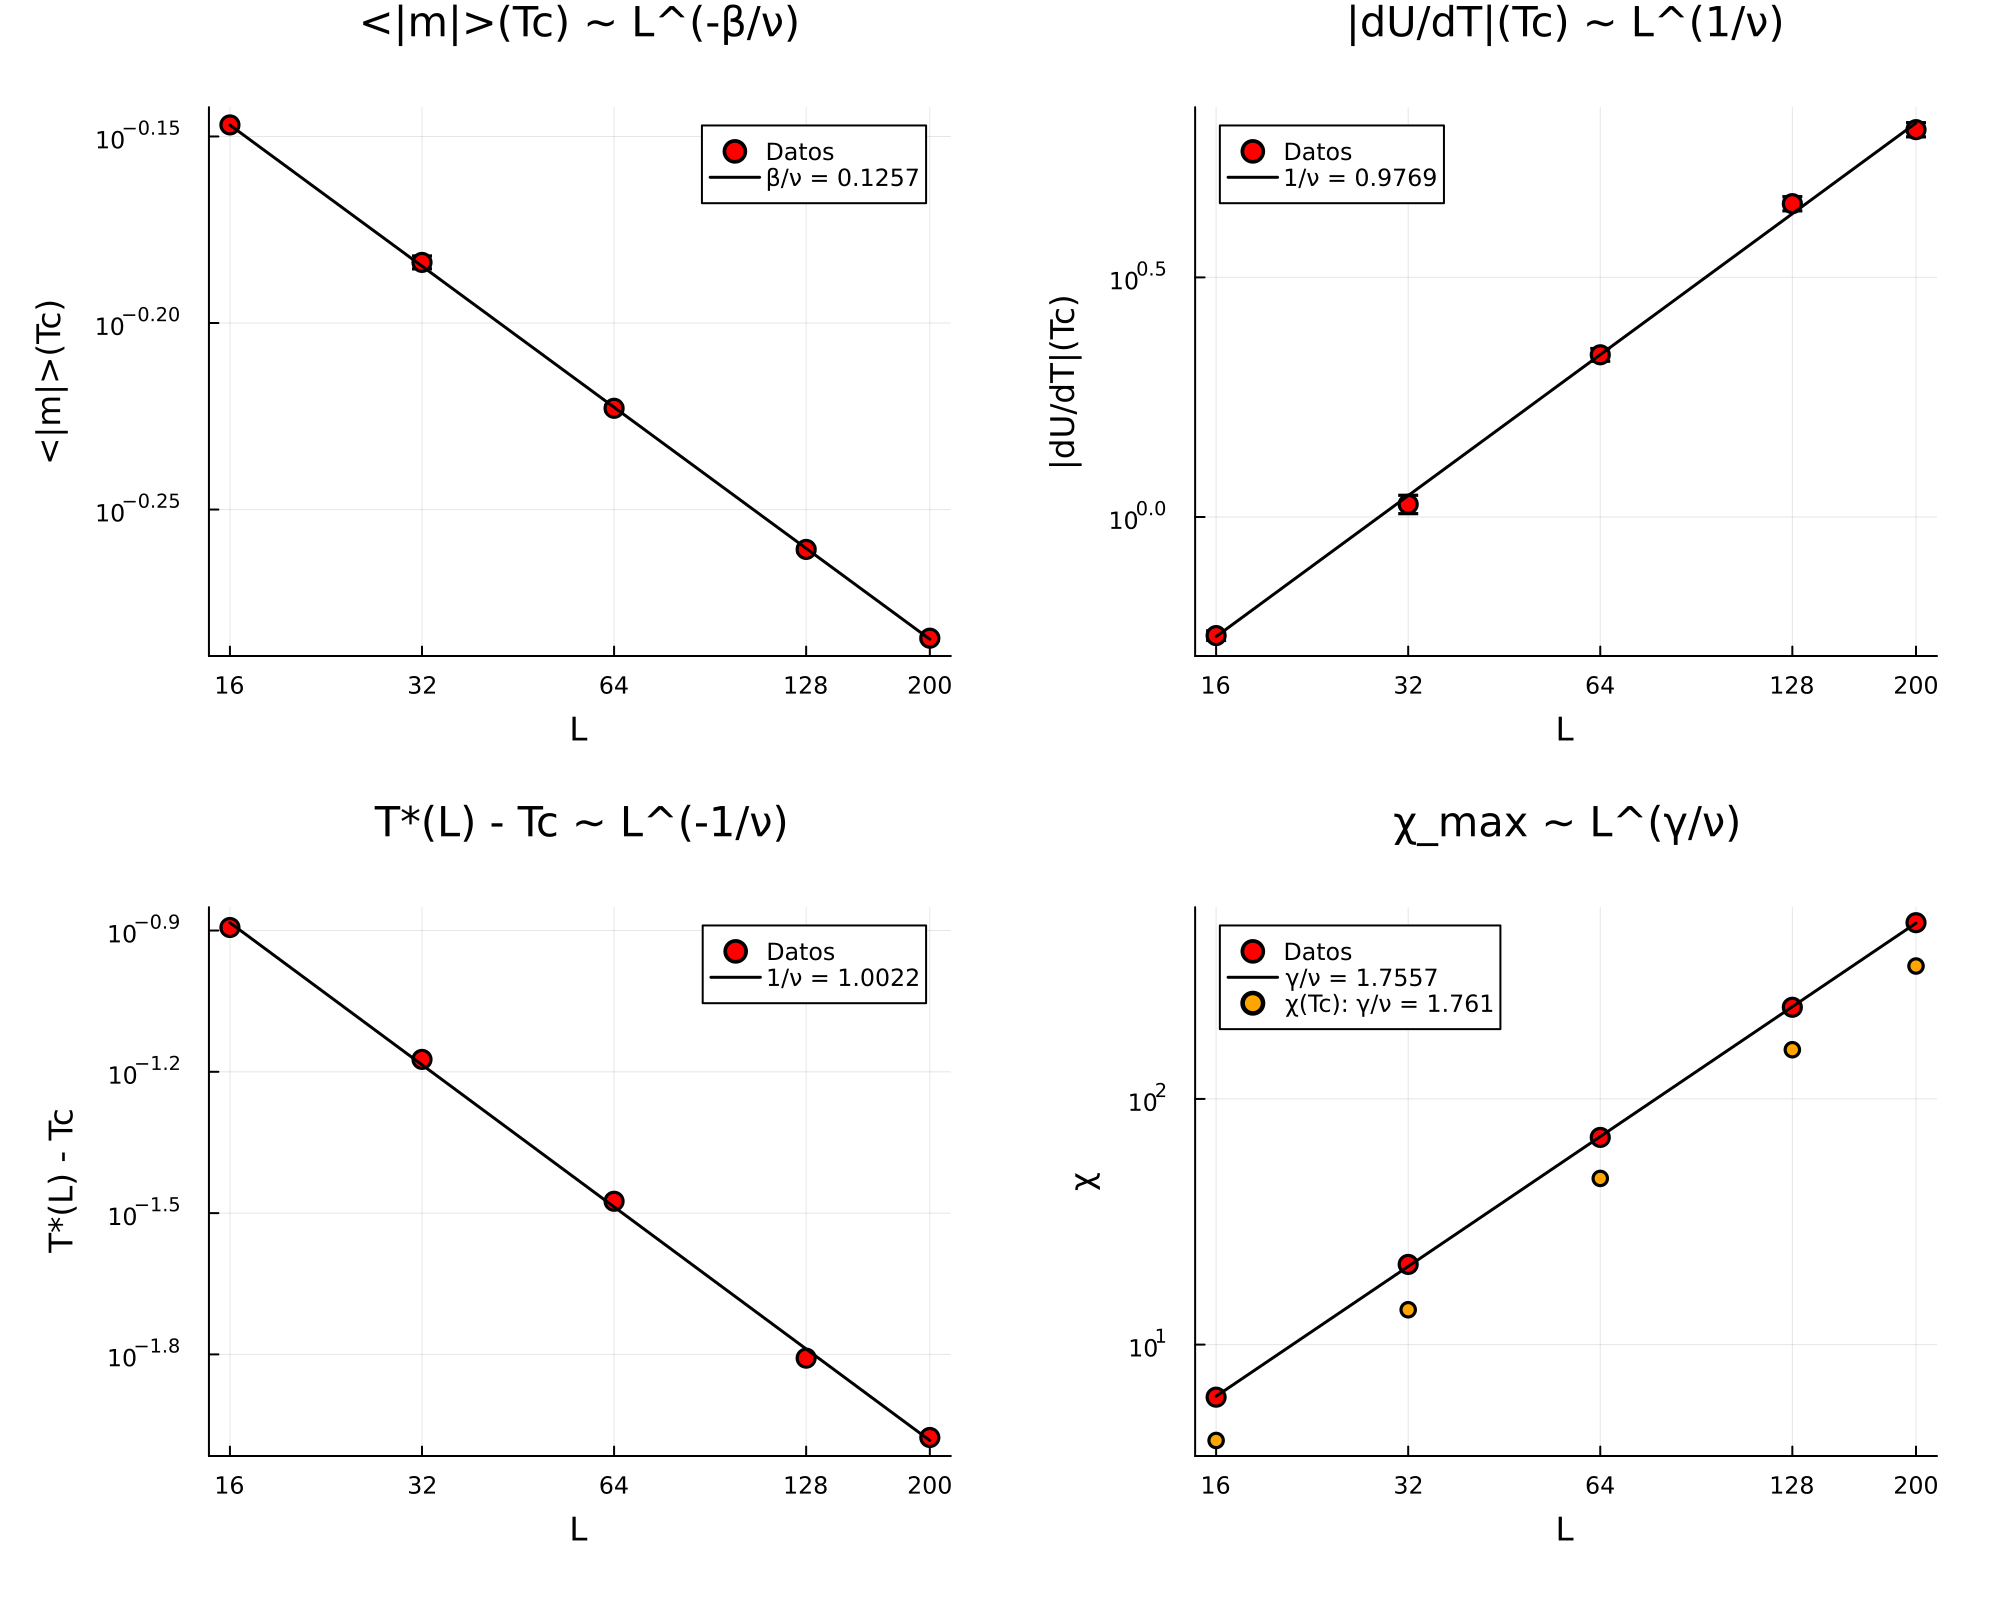
\includegraphics[width=\textwidth]{critical_exponents_fss.png}
  \caption{\todo{Ajustes de FSS en $\Tc$.}}
  \label{fig:exponentes}
\end{figure}

\begin{table}[htbp]
  \centering
  \caption{\todo{Exponentes críticos estimados y exactos.}}
  \label{tab:exponentes}
  \begin{tabular}{lccc}
    \toprule
    Exponente & Relación & Estimado & Exacto \\
    \midrule
    $\nu$    & FSS de $dU_L/dT$          & \todo{} & $1$ \\
    $\beta$  & $\nu \cdot (\beta/\nu)$   & \todo{} & $1/8$ \\
    $\gamma$ & $\nu \cdot (\gamma/\nu)$  & \todo{} & $7/4$ \\
    $\alpha$ & $2 - d\nu$                & \todo{} & $0$ (log) \\
    $\eta$   & $2 - \gamma/\nu$          & \todo{} & $1/4$ \\
    $\delta$ & $1 + \gamma/\beta$        & \todo{} & $15$ \\
    \bottomrule
  \end{tabular}
\end{table}

\subsection{Magnetización en función del campo}
\label{sec:campo}
\todo{Ítem (f): curvas $m(B)$, exponente $\delta$ y colapso $m/|t|^\beta$ vs $B/|t|^\Delta$.}

\begin{figure}[htbp]
  \centering
  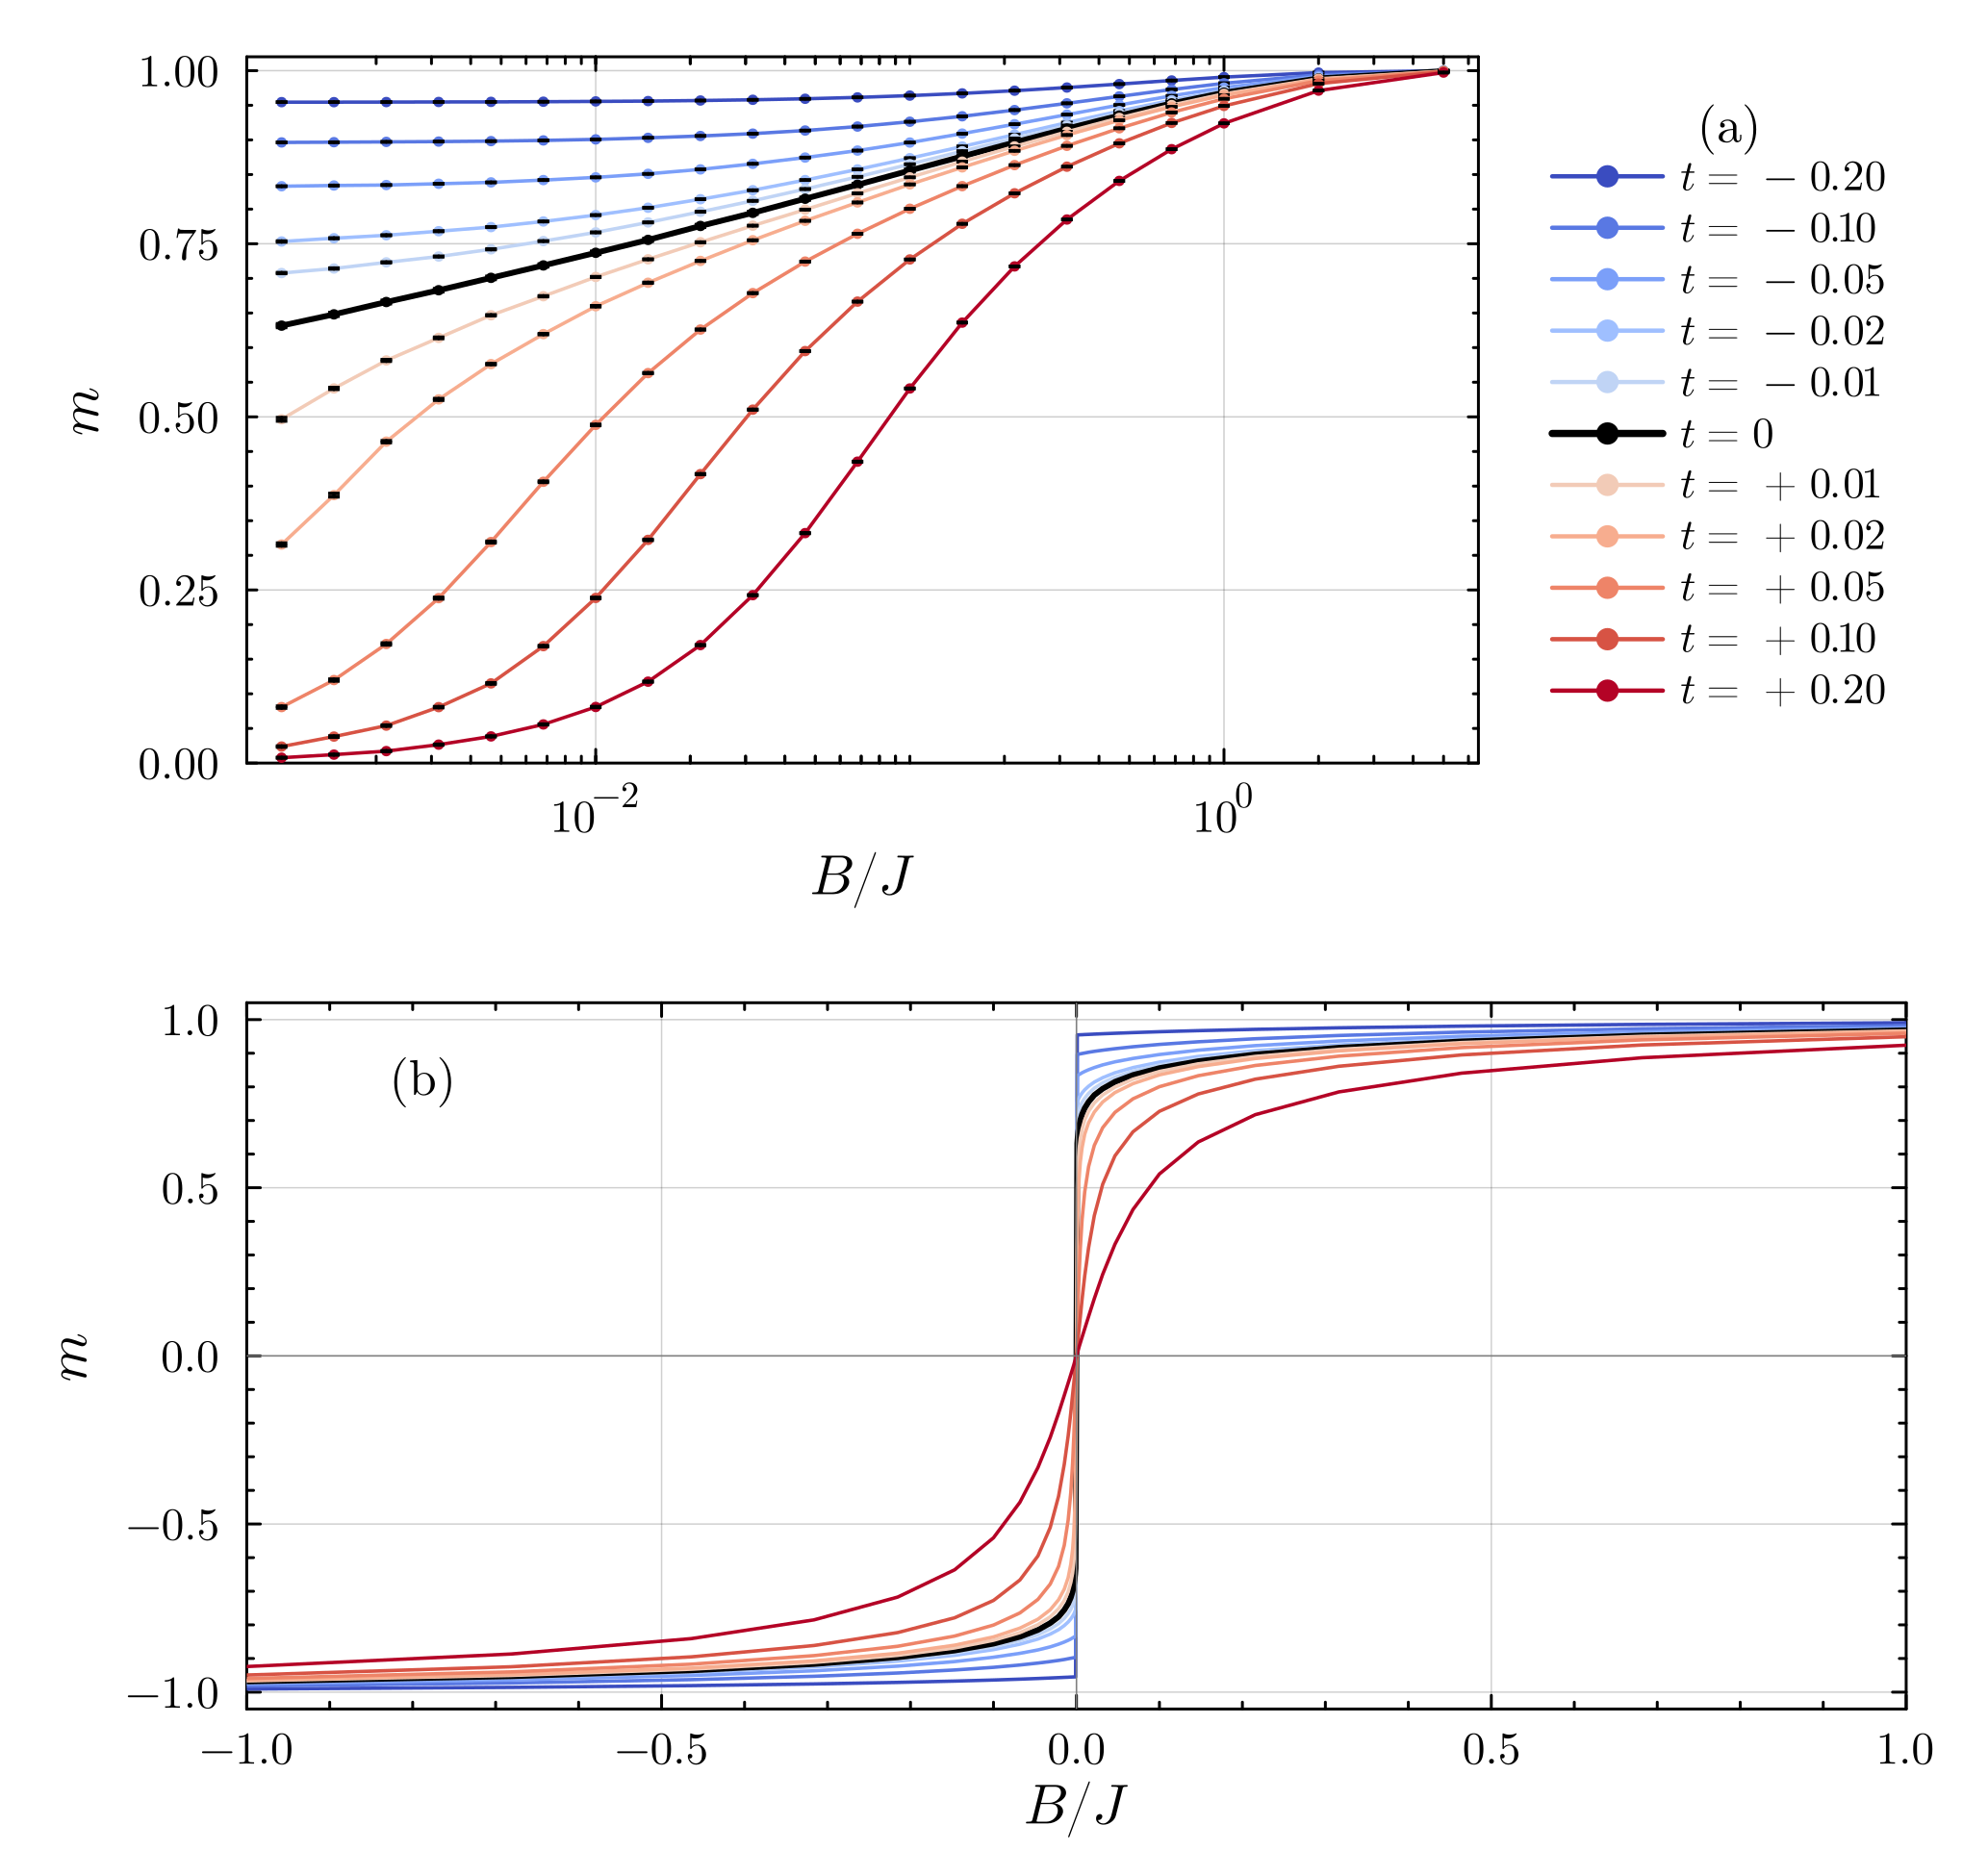
\includegraphics[width=\textwidth]{field_magnetization_curves.png}
  \caption{\todo{$m(B/J)$ para distintas temperaturas.}}
  \label{fig:campo}
\end{figure}

\begin{figure}[htbp]
  \centering
  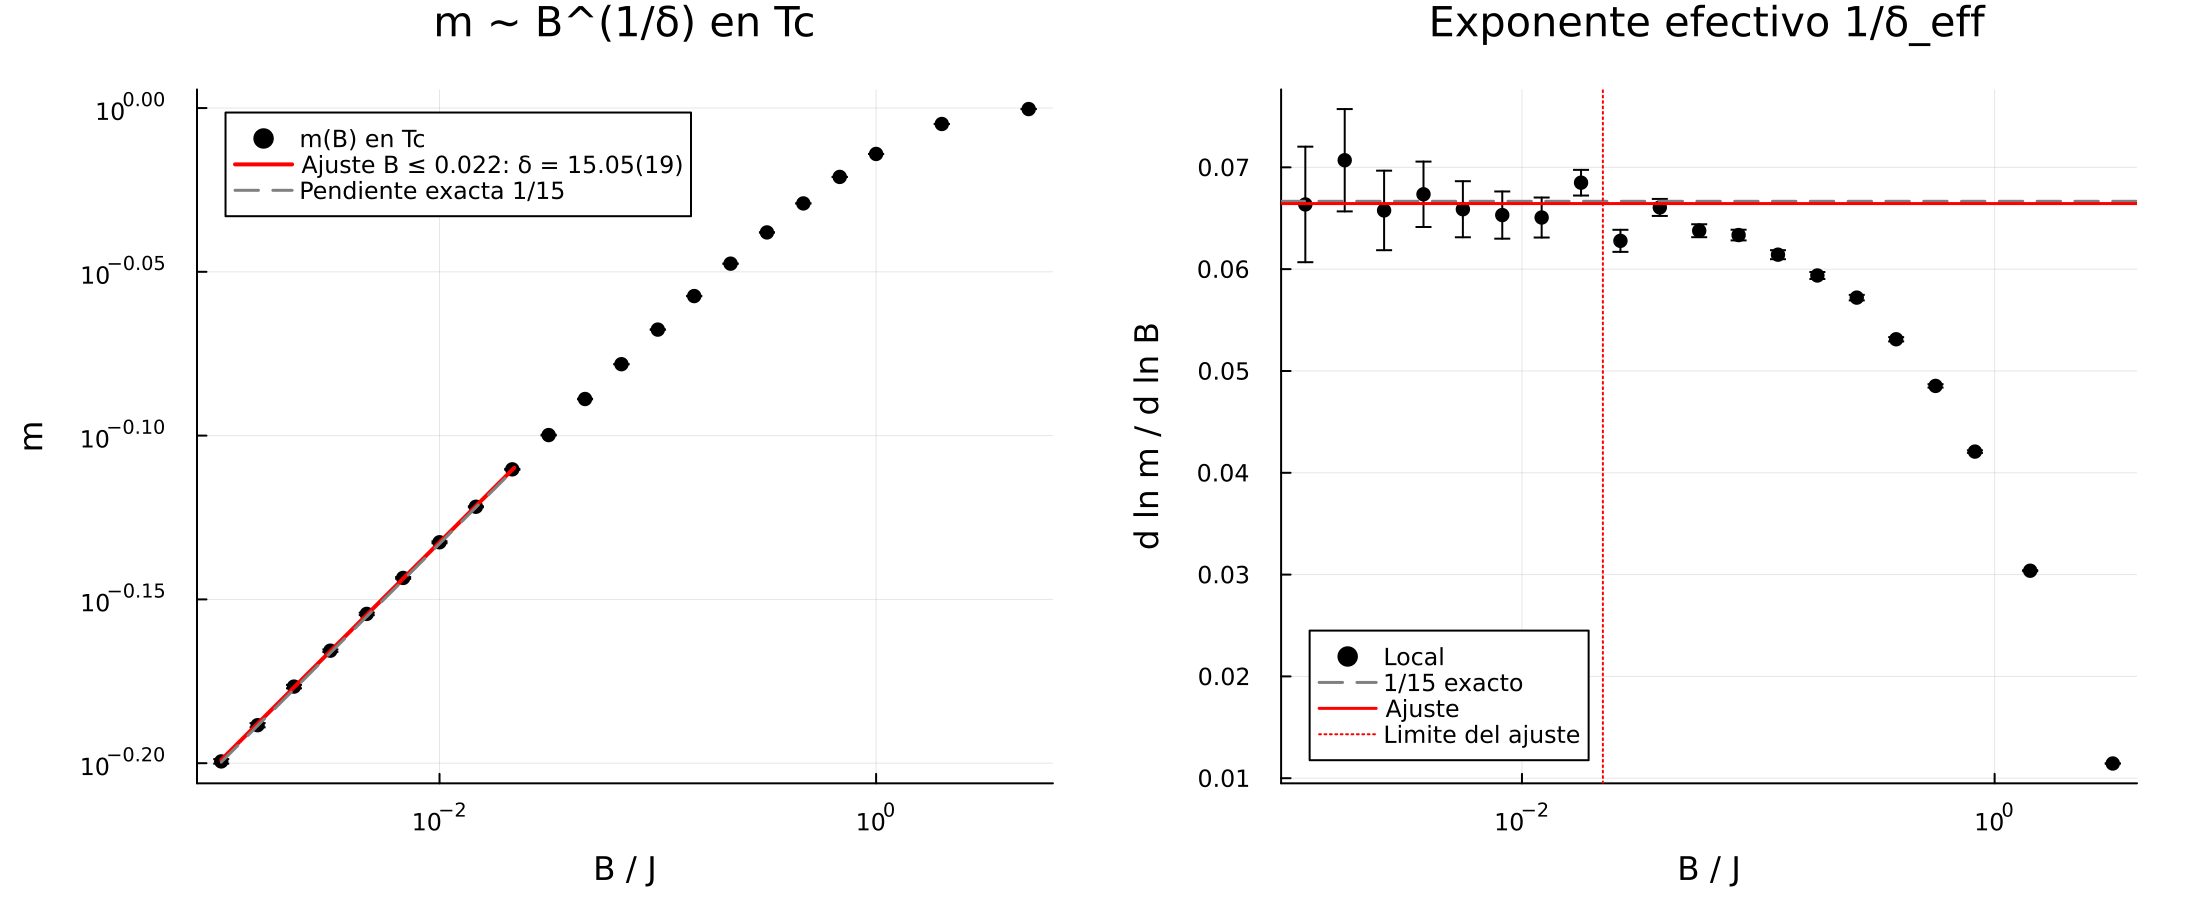
\includegraphics[width=\textwidth]{field_delta.png}
  \caption{\todo{Estimación de $\delta$ en $\Tc$.}}
  \label{fig:delta}
\end{figure}

\begin{figure}[htbp]
  \centering
  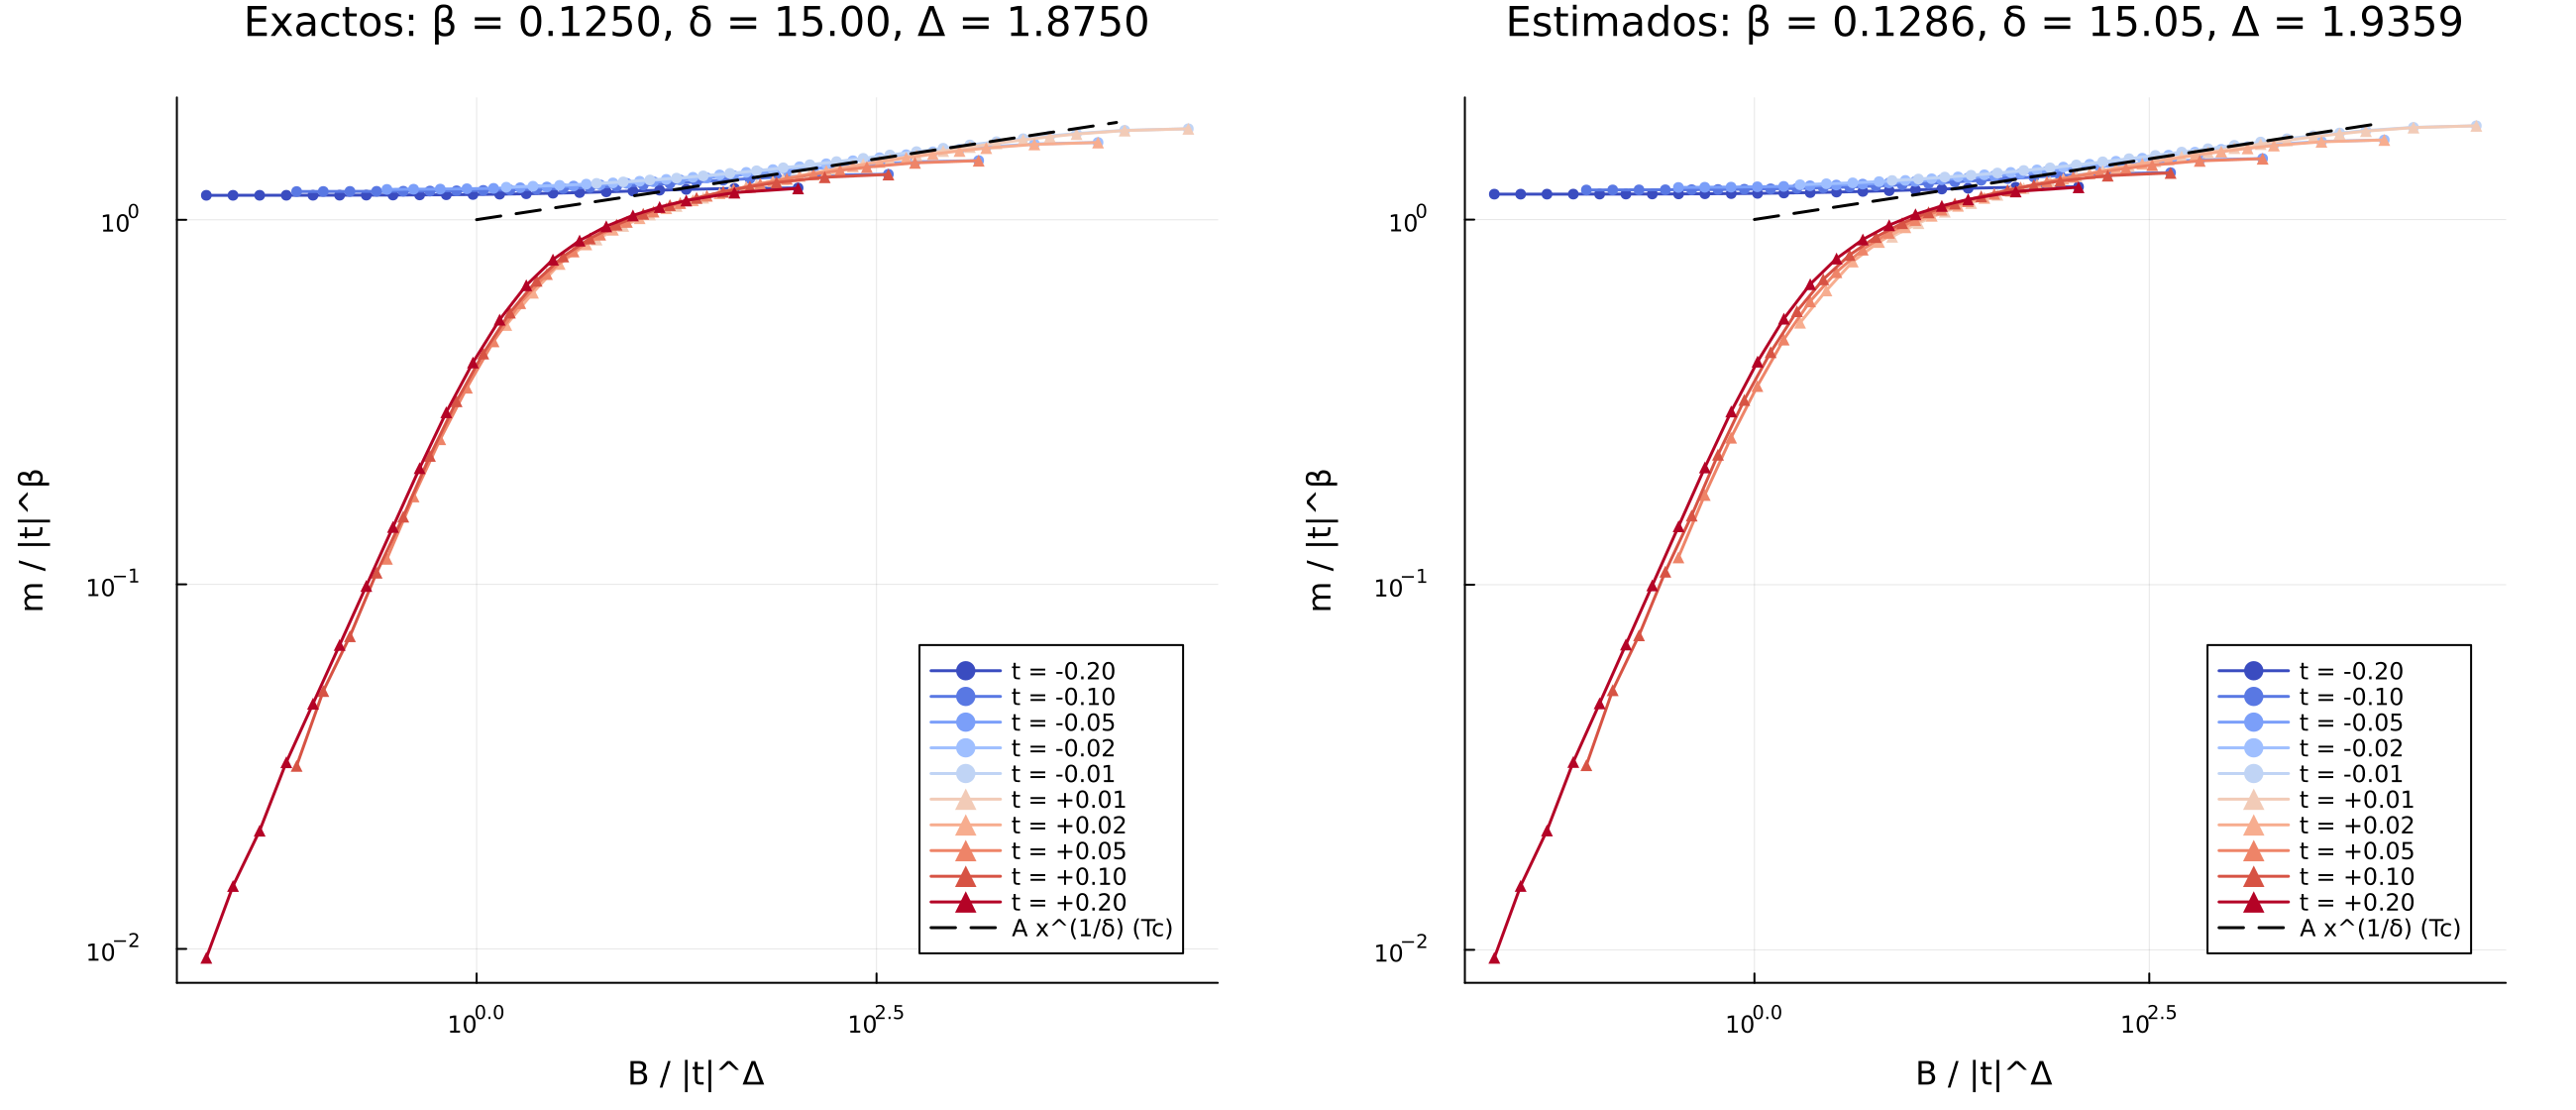
\includegraphics[width=\textwidth]{field_scaling_collapse.png}
  \caption{\todo{Colapso con exponentes exactos y estimados.}}
  \label{fig:colapso}
\end{figure}

\subsection{Calor específico}
\label{sec:cv}
\todo{Ítem (g): $\max C \sim L^{\alpha/\nu}$ frente a divergencia logarítmica.}

\begin{figure}[htbp]
  \centering
  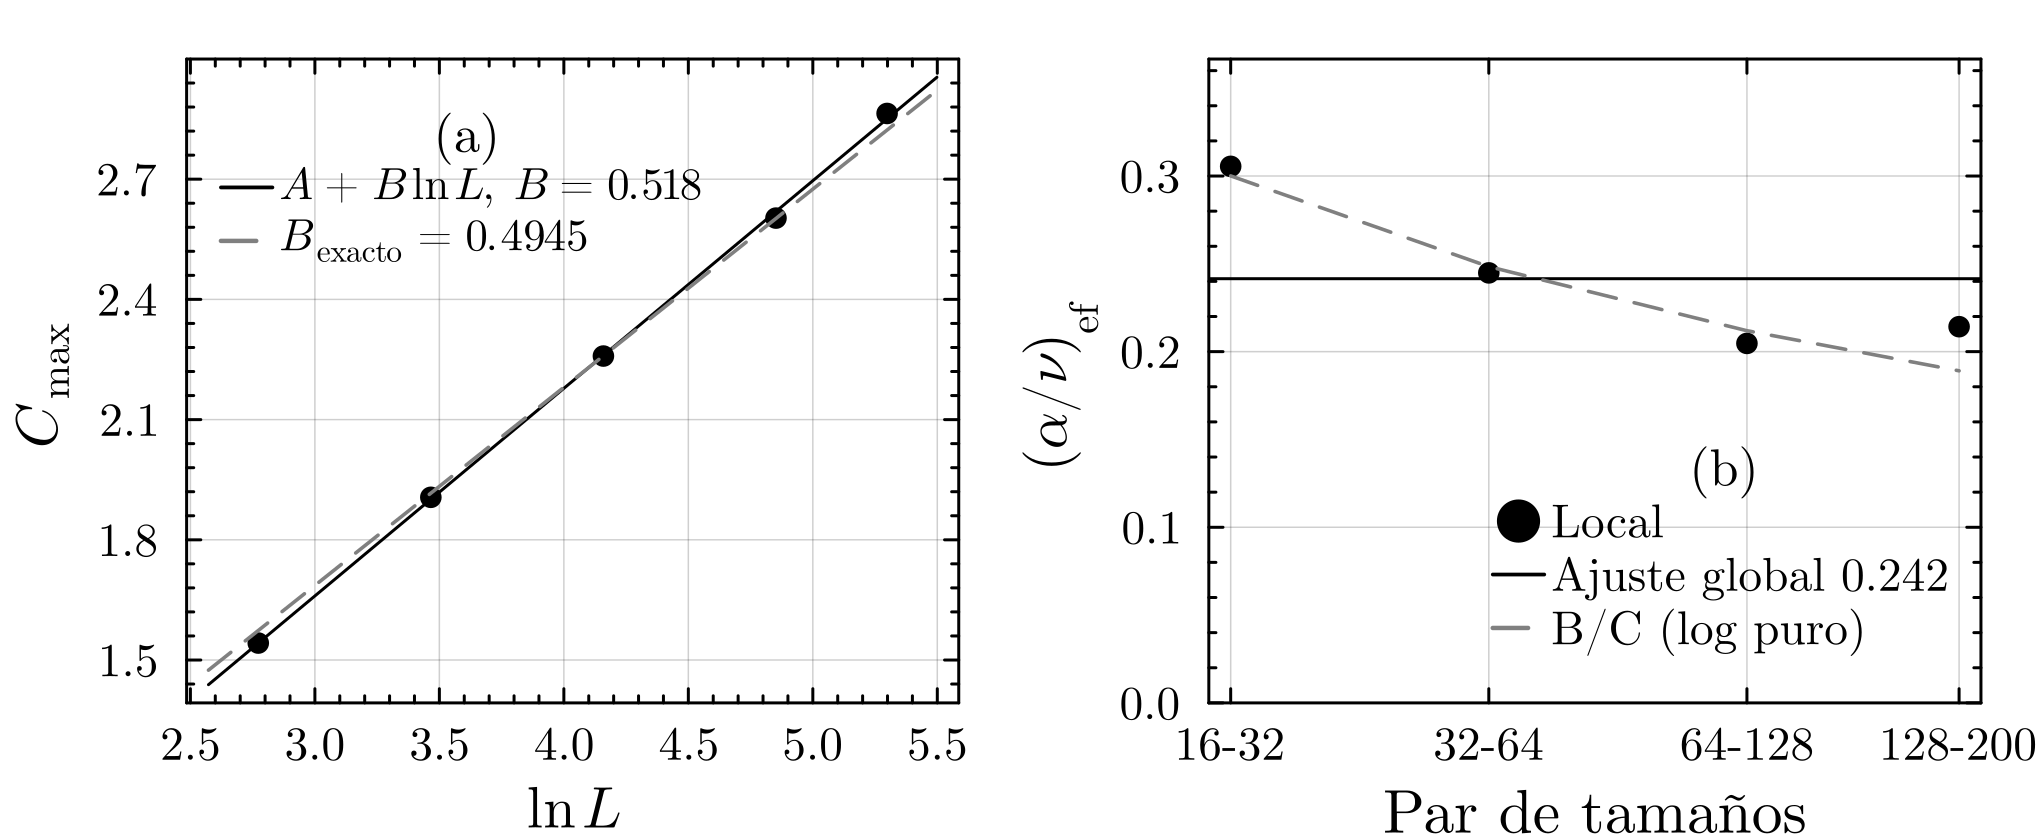
\includegraphics[width=\textwidth]{specific_heat_scaling.png}
  \caption{\todo{Crecimiento de $C_\mathrm{max}$ con $L$.}}
  \label{fig:cv}
\end{figure}

\subsection{Resumen de las estimaciones de $\Tc$}
\begin{table}[htbp]
  \centering
  \caption{\todo{Estimaciones de la temperatura crítica.}}
  \label{tab:Tc}
  \begin{tabular}{lc}
    \toprule
    Método & $\Tc$ \\
    \midrule
    Inflexión de $\expval{|m|}$             & \todo{} \\
    Cruce de Binder                        & \todo{} \\
    Máximo de $\chi$, $T^*(L) \to \Tc$     & \todo{} \\
    Exacto (Onsager)                       & $2/\ln(1+\sqrt{2}) = 2.269185\ldots$ \\
    \bottomrule
  \end{tabular}
\end{table}

% =========================================================================
\section{Conclusiones}
% =========================================================================
\todo{}

% =========================================================================
\printbibliography

\end{document}
